\documentclass[12pt,a4paper]{article}

% ---------- PAQUETES ----------
\usepackage[spanish,es-nodecimaldot]{babel}
\usepackage[utf8]{inputenc}
\usepackage[T1]{fontenc}
\usepackage[a4paper,margin=2.5cm]{geometry}
\usepackage{graphicx}
\usepackage{xcolor}
\usepackage{parskip}
\usepackage{csquotes}
\usepackage[backend=bibtex,style=ieee]{biblatex}

\addbibresource{referencias.bib}

\linespread{1.15}\selectfont
\setlength{\parindent}{0pt}

% Anchos de numeración del índice
\makeatletter
\renewcommand*\l@section{\@dottedtocline{1}{0em}{2.5em}}
\renewcommand*\l@subsection{\@dottedtocline{2}{2.5em}{3.5em}}
\renewcommand*\l@subsubsection{\@dottedtocline{3}{6em}{4.5em}}
\makeatother

% ---------- DOCUMENTO ----------
\begin{document}

\begin{titlepage}
    \centering
    \vspace*{1.2cm}

    {\fontsize{22}{27}\selectfont\bfseries
    Chidori: Diseño, desarrollo e investigación de un equipo médico de medición de
    bioimpedancia vesical para la prevención de eventos de incontinencia urinaria\par}

    \vspace{1.4cm}

    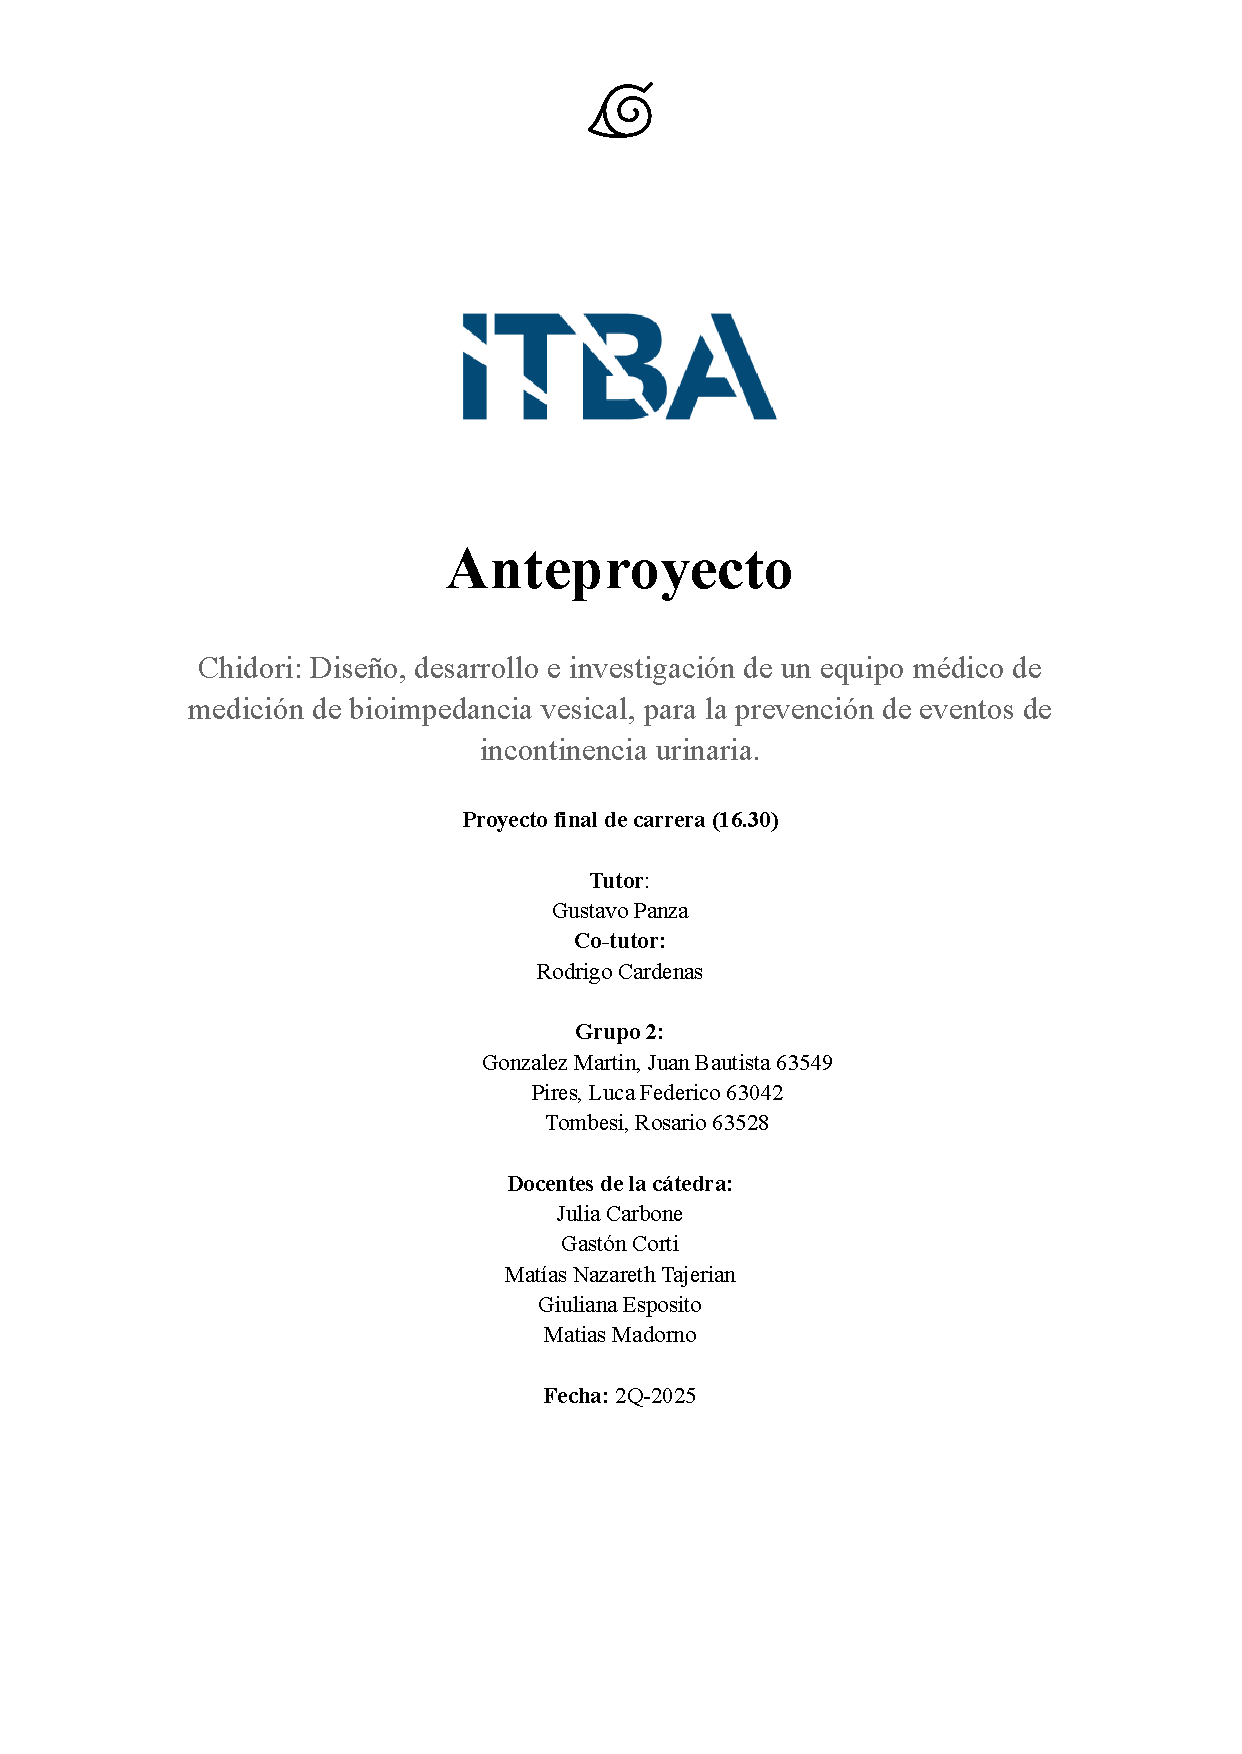
\includegraphics[page=1,viewport=180 615 415 715,clip,width=0.35\textwidth]
    {Anteproyecto.pdf}

    \vspace{1.5cm}

    {\normalsize\itshape
    Proyecto final de Carrera para la obtención del título de Bioingeniero\par}

    \vspace{1.2cm}

    {\large
    \textbf{Autores:}\par
    Gonzalez Martin, Juan Bautista (63549)\par
    Pires, Luca Federico (63042)\par
    Tombesi, Rosario (63528)\par}

    \vspace{1.2cm}

    {\large
    \textbf{Tutor:} Gustavo Panza\par
    \vspace{0.35cm}
    \textbf{Co-tutor:} Dante Kienigiel\par}

    \vfill

    \begin{flushleft}
        {\large Fecha de entrega: }
    \end{flushleft}
\end{titlepage}

\pagenumbering{roman}
\tableofcontents
\clearpage

\pagenumbering{arabic}

\section{Introducción}

\subsection{Motivación}

La incontinencia urinaria es la pérdida involuntaria de orina y constituye una condición que
puede afectar a personas de todas las edades, con un impacto significativo sobre la salud, la
autonomía y la calidad de vida de quienes la padecen \cite{abrams2002standardisation}. Esta
afección presenta una alta prevalencia en la población adulta y es entre dos y cuatro veces más
frecuente en mujeres que en hombres. Además, su incidencia aumenta progresivamente con la edad
y, debido a su elevada prevalencia e impacto negativo en personas mayores de 65 años, es
considerada un síndrome geriátrico \cite{robles2006incontinencia}.

Si bien la incontinencia urinaria se asocia con mayor frecuencia al envejecimiento, puede
presentarse en individuos de cualquier grupo etario. En las mujeres, el embarazo, el parto y la
menopausia constituyen factores de riesgo relevantes, mientras que en los hombres suele asociarse
con patologías prostáticas. Asimismo, diversas enfermedades neurológicas, como las lesiones
medulares, la esclerosis múltiple y la enfermedad de Parkinson, pueden alterar el control vesical
y favorecer la aparición de esta condición \cite{leslie2024incontinence}.

Las terapias y los tratamientos utilizados actualmente en pacientes con incontinencia urinaria
pueden clasificarse en distintas categorías complementarias entre sí. En primer lugar, se
encuentran las terapias conservadoras, orientadas a disminuir los síntomas mediante modificaciones
en el estilo de vida. Entre las principales medidas se incluyen cambios en la dieta, abandono del
tabaquismo, descenso de peso y ejercicios de fortalecimiento del suelo pélvico. Asimismo, suelen
implementarse micciones programadas con el objetivo de prevenir episodios de incontinencia. Sin
embargo, aunque estas estrategias pueden resultar efectivas en ciertos casos, los horarios fijos
pueden ser rígidos y poco adaptables a las necesidades particulares y al contexto cotidiano de
cada paciente.

En segundo lugar, existen tratamientos farmacológicos, principalmente indicados ante determinados
síntomas de urgencia. Los fármacos utilizados incluyen antimuscarínicos y agonistas $\beta_3$, los
cuales pueden contribuir a reducir los episodios de incontinencia. No obstante, su uso puede
asociarse con efectos adversos, especialmente relevantes en adultos mayores, como sequedad bucal,
constipación, visión borrosa y mareos \cite{eau2025femaleLUTS}.

Finalmente, cuando las alternativas conservadoras y farmacológicas no resultan efectivas, pueden
considerarse procedimientos invasivos. Según el tipo de incontinencia y la condición del paciente,
estos incluyen la neuromodulación sacra, la administración intravesical de toxina botulínica y
distintas cirugías correctivas. Si bien estos procedimientos pueden mejorar significativamente los
síntomas, algunos se caracterizan por ser costosos, invasivos y estar asociados con posibles
complicaciones \cite{eau2025femaleLUTS}.

En la práctica clínica, especialmente en pacientes adultos mayores, es frecuente recurrir a
productos absorbentes como estrategia de contención. Sin embargo, esta solución también presenta
limitaciones, ya que puede representar una carga económica sostenida y no aborda el mecanismo que
origina la pérdida de orina.

A pesar de la variedad de tratamientos disponibles, persisten desafíos asociados con su
implementación y efectividad a largo plazo. Muchas alternativas presentan limitaciones vinculadas
con su costo, invasividad, efectos adversos o escasa adaptabilidad a pacientes con movilidad
reducida o deterioro cognitivo. Estas dificultades evidencian la necesidad de desarrollar nuevas
estrategias que permitan mejorar el monitoreo y la gestión de la condición de manera accesible,
segura y adaptada a las necesidades de cada paciente.

En este contexto, la bioimpedancia eléctrica surge como una alternativa prometedora para el
monitoreo no invasivo y continuo del estado vesical. Esta técnica se basa en la medición de las
propiedades eléctricas de los tejidos biológicos mediante la inyección de corrientes alternas de
baja amplitud y el análisis de la respuesta eléctrica obtenida. Debido a que los tejidos y fluidos
corporales presentan propiedades eléctricas diferentes, los cambios en el volumen de orina dentro
de la vejiga pueden producir variaciones medibles en la impedancia eléctrica de la región abdominal
\cite{abbey1983bladder,liao2011bladder}.

El desarrollo de dispositivos portátiles basados en bioimpedancia podría permitir la implementación
de sistemas de monitoreo continuo, de bajo costo y potencialmente utilizables en entornos
domiciliarios o clínicos. No obstante, la medición de bioimpedancia vesical presenta desafíos
relacionados con la variabilidad anatómica entre individuos, el movimiento corporal, la ubicación
de los electrodos y la influencia de otros tejidos abdominales sobre la señal obtenida
\cite{palla2023review}.

El presente proyecto propone estudiar la bioimpedancia como herramienta no invasiva para estimar el
estado de llenado vesical y anticipar la necesidad de micción. Su relevancia radica en aportar
evidencia científica sobre un enfoque accesible, continuo y objetivo, con potencial para mejorar el
manejo de pacientes con incontinencia urinaria. El trabajo parte de un prototipo desarrollado
previamente y aborda su rediseño electrónico, la mejora de la calidad de señal, la recolección
experimental de datos y la evaluación de métodos de predicción personalizados.

\subsection{Objetivos}

\subsubsection{Objetivo general}

Desarrollar y validar un dispositivo médico portátil y económico para el monitoreo no invasivo del
llenado vesical mediante bioimpedancia eléctrica, optimizando un prototipo existente y realizando un
estudio experimental orientado a la generación de una base de datos poblacional que permita analizar
la relación entre la impedancia y el volumen vesical, así como explorar técnicas de predicción del
momento de la micción para la prevención de episodios de incontinencia urinaria.

\subsubsection{Objetivos específicos}

El presente trabajo tiene como objetivo el rediseño y la optimización de un sistema de medición de
bioimpedancia orientado al monitoreo del llenado vesical. Para ello, se propone desarrollar una nueva
placa electrónica que incorpore un esquema de filtrado en la etapa de adquisición de la señal, con el
fin de reducir el nivel de ruido y mejorar la sensibilidad y estabilidad general del dispositivo.
Asimismo, se buscará optimizar la portabilidad del sistema mediante la reducción del consumo
energético y del tamaño de la placa electrónica.

Además, se plantea desarrollar una interfaz gráfica que facilite la interacción con el usuario y
permita una visualización clara e intuitiva de los resultados. En paralelo, se construirá una base
de datos experimental a partir de mediciones obtenidas durante pruebas controladas. Esta base
permitirá implementar y evaluar modelos de análisis de datos orientados a predecir el estado de
llenado vesical a partir de cambios en la bioimpedancia.

El trabajo también tiene como finalidad investigar y definir métricas cuantitativas para evaluar la
confiabilidad, estabilidad y desempeño del sistema, estableciendo criterios objetivos para su
validación. Se buscará realizar pruebas experimentales en distintos escenarios de uso con el propósito
de analizar la seguridad y eficacia del sistema, considerando su potencial aplicación clínica. Como
objetivo de máxima, se propone publicar los resultados obtenidos en una revista científica o congreso
relacionado con las áreas de bioingeniería y bioimpedancia.

\section{Marco teórico}

\subsection{Vejiga urinaria}

\subsubsection{Anatomía y fisiología}

La vejiga urinaria es un órgano muscular hueco ubicado en la cavidad pélvica y constituye la víscera
más anterior de la pelvis. Su función principal es almacenar temporalmente la orina producida por los
riñones hasta que pueda ser eliminada mediante la micción. Cuando se encuentra vacía permanece dentro
de la pelvis, por detrás de la sínfisis del pubis; a medida que se llena, se distiende y asciende hacia
la cavidad abdominal \cite{drake2015gray,shermadou2023bladder}.

En estado de vaciamiento presenta una forma aproximadamente piramidal y puede describirse mediante un
vértice, una base o fondo, un cuerpo y un cuello. El vértice se orienta hacia la sínfisis del pubis y
se continúa con el ligamento umbilical medio, remanente del uraco que se dirige hacia el ombligo. La
base se orienta en dirección posteroinferior y el cuerpo constituye la región principal de
almacenamiento. Inferiormente, la vejiga se estrecha para formar el cuello vesical, que se continúa con
la uretra \cite{drake2015gray,shermadou2023bladder}.

Los dos uréteres ingresan por la región posterior de la vejiga y la uretra se origina en su extremo
inferior. Los orificios ureterales y el orificio uretral interno delimitan sobre la superficie interna
una región triangular denominada trígono vesical. El trayecto oblicuo de los uréteres a través de la
pared vesical contribuye a limitar el reflujo de orina hacia el tracto urinario superior cuando la
vejiga se llena o se contrae durante la micción \cite{lanzotti2023physiology}. Esta pared se encuentra
revestida internamente por urotelio y contiene una capa de músculo liso denominada músculo detrusor,
cuya contracción coordinada permite expulsar la orina \cite{drake2015gray}.

La función vesical comprende una fase de almacenamiento y otra de vaciamiento o micción. Durante el
llenado, la distensibilidad de la pared permite que el volumen aumente con una elevación relativamente
pequeña de la presión intravesical, propiedad denominada acomodación o \textit{compliance} vesical. La
capacidad funcional varía entre individuos; en el adulto, el volumen que puede almacenarse cómodamente
es, en promedio, de 300 a 400~mL \cite{drake2015gray,lanzotti2023physiology}.

A medida que la vejiga se llena, la distensión de su pared activa receptores sensitivos que informan
el estado de llenado a la médula espinal y a los centros encefálicos. Durante el almacenamiento, la
actividad simpática y somática mantiene relajado el detrusor y cerrada la salida uretral. Cuando el
grado de llenado y el contexto permiten iniciar la micción, aumenta la actividad parasimpática, se
contrae el detrusor y disminuye la resistencia uretral. Esto requiere la relajación coordinada del
cuello vesical y del esfínter uretral externo, este último formado por músculo estriado y sujeto al
control voluntario. De este modo, circuitos espinales y encefálicos coordinan la expulsión de la orina
\cite{fowler2008neural,lanzotti2023physiology}.


\subsubsection{Incontinencia urinaria}

La International Continence Society define la incontinencia urinaria como la queja de cualquier pérdida
involuntaria de orina \cite{abrams2002standardisation}. Se trata de un síntoma y no de una etiología
única. Las formas clínicas más frecuentes son:

\begin{itemize}
    \item \textbf{Incontinencia urinaria de esfuerzo:} pérdida asociada con un esfuerzo, ejercicio,
    tos o estornudo, generalmente vinculada con hipermovilidad uretral o insuficiencia esfinteriana.
    \item \textbf{Incontinencia urinaria de urgencia:} pérdida precedida o acompañada por una necesidad
    súbita y difícil de posponer. Puede presentarse dentro del síndrome de vejiga hiperactiva.
    \item \textbf{Incontinencia mixta:} coexistencia de síntomas de esfuerzo y de urgencia.
    \item \textbf{Incontinencia por rebosamiento o asociada con retención:} pérdida relacionada con un
    vaciado insuficiente y un volumen residual elevado.
    \item \textbf{Incontinencia funcional:} incapacidad de llegar al sanitario o utilizarlo a tiempo
    por limitaciones motoras, cognitivas o ambientales, aun cuando el tracto urinario pueda conservar
    su función.
\end{itemize}

Desde el punto de vista fisiopatológico, la incontinencia puede deberse a alteraciones del detrusor o
del tracto de salida vesical. Entre las primeras se encuentran la hiperactividad del detrusor y la
disminución de la acomodación; entre las segundas, la hipermovilidad uretral y la incompetencia
esfinteriana. Por ello, la pérdida involuntaria de orina debe entenderse como un síntoma que puede
responder a mecanismos y enfermedades diferentes, cuya identificación es necesaria para orientar el
tratamiento \cite{chiang2013incontinencia}.

El monitoreo del llenado no corrige por sí mismo la causa de la incontinencia; busca aportar una señal anticipatoria para personas que
conservan capacidad de almacenamiento y pueden beneficiarse de una indicación de vaciado. Esto puede
ser especialmente útil cuando la percepción de plenitud está disminuida.


\subsubsection{Tratamientos y estrategias de manejo actuales}

El abordaje se selecciona según el subtipo, la gravedad, las comorbilidades y las preferencias del
paciente. Las intervenciones conservadoras suelen constituir la primera línea e incluyen educación,
ajustes en la ingesta de líquidos, reducción de peso cuando está indicada, entrenamiento vesical y
ejercicios supervisados de la musculatura del piso pélvico. Existe evidencia de beneficio del
entrenamiento del piso pélvico en mujeres con incontinencia de esfuerzo y mixta
\cite{eau2025femaleLUTS,dumoulin2018pelvic}.

En la incontinencia de urgencia pueden emplearse antimuscarínicos o agonistas $\beta_3$. La elección
requiere valorar contraindicaciones, adherencia y efectos adversos, particularmente en personas mayores.
Cuando las medidas previas son insuficientes se consideran, según el cuadro, toxina botulínica
intradetrusor, neuromodulación, agentes de relleno uretral o procedimientos quirúrgicos. Los productos
absorbentes y la micción asistida o programada ayudan a contener o prevenir episodios, pero no tratan
necesariamente el mecanismo subyacente \cite{eau2025femaleLUTS}.

El intervalo entre micciones cambia con la ingesta, la diuresis, la actividad y
otros factores. Una estimación continua del llenado mediante bioimpedancia podría permitir avisos personalizados; su utilidad
clínica, sin embargo, deberá demostrarse mediante estudios comparativos y no puede inferirse únicamente
del desempeño electrónico.

\subsection{Bioimpedancia eléctrica}

\subsubsection{Principios generales}

La bioimpedancia caracteriza la oposición que presenta un tejido al paso de corriente.
Para una excitación sinusoidal en régimen estacionario, se define como

\begin{equation}
    Z(\omega)=\frac{\underline{V}(\omega)}{\underline{I}(\omega)}
             =R(\omega)+jX(\omega),
\end{equation}

donde $R$ es la componente resistiva, $X$ la reactancia y $\omega=2\pi f$. Su módulo y fase resultan

\begin{equation}
    |Z|=\sqrt{R^2+X^2}, \qquad
    \phi=\tan^{-1}\left(\frac{X}{R}\right).
\end{equation}

Los líquidos intra y extracelulares aportan caminos conductivos, mientras que las membranas celulares
se comportan aproximadamente como elementos capacitivos. Por esta razón la impedancia depende de la
frecuencia. A bajas frecuencias la corriente circula principalmente por el espacio extracelular; al
aumentar la frecuencia, la reactancia de membrana disminuye y una fracción mayor atraviesa el medio
intracelular \cite{grimnes2015bioimpedance}. El tejido es heterogéneo y anisótropo, de modo que un
modelo concentrado representa un comportamiento macroscópico y no una descripción anatómica exacta.

El modelo equivalente presentado por Al-Rawi et al. representa el medio extracelular mediante
$R_o$ y el intracelular mediante $R_i$, mientras que $C_{in}$ modela el comportamiento capacitivo de
la membrana celular. Esta disposición permite visualizar cómo el aumento de la frecuencia reduce la
reactancia capacitiva y habilita una mayor contribución del camino intracelular
\cite{alrawi2013howland}.

\begin{figure}[htbp]
    \centering
    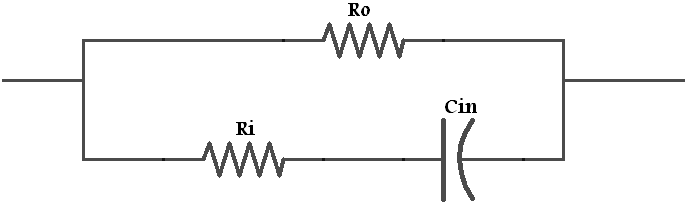
\includegraphics[width=0.70\textwidth]{figuras/alrawi2013/modelo-equivalente.png}
    \caption{Modelo eléctrico equivalente simplificado del tejido biológico. $R_o$ representa la
    resistencia extracelular, $R_i$ la resistencia intracelular y $C_{in}$ la capacitancia de la
    membrana celular. Reproducida de Al-Rawi et al. \cite{alrawi2013howland}.}
    \label{fig:modelo_equivalente_alrawi}
\end{figure}

Una representación habitual es el modelo de Cole--Cole:

\begin{equation}
 Z(\omega)=R_{\infty}+\frac{R_0-R_{\infty}}
 {1+(j\omega\tau)^{1-\alpha}},
\end{equation}

donde $R_0$ y $R_{\infty}$ son los límites resistivos de baja y alta frecuencia, $\tau$ es una constante
de tiempo y $\alpha$ describe la dispersión de los tiempos de relajación \cite{cole1940permeability}.
Este modelo es especialmente útil en espectroscopía. En una medición a frecuencia única, se sigue la 
evolución temporal de un punto del espectro y no es posible identificar de forma independiente todos sus parámetros.

\subsubsection{Métodos de medición}

La medición de impedancia eléctrica en el cuerpo se realiza principalmente mediante el método
corriente--tensión: se inyecta una corriente alterna de amplitud conocida y se mide la tensión
resultante sobre la superficie corporal. Según la cantidad y función de los electrodos, pueden
distinguirse tres configuraciones \cite{noyori2022review}:

\begin{itemize}
    \item \textbf{Bipolar:} utiliza dos electrodos, ambos compartidos para inyectar corriente y medir
    tensión. Es la configuración más simple y compacta, pero la impedancia medida incluye directamente
    las interfaces electrodo--piel.
    \item \textbf{Tripolar:} emplea un electrodo de corriente, uno de tensión y un tercero común a
    ambas funciones. Permite medir el potencial en un punto distinto del de inyección y conserva una
    implementación relativamente sencilla, aunque el electrodo compartido mantiene la influencia de
    la impedancia de contacto.
    \item \textbf{Tetrapolar:} utiliza dos electrodos para inyectar corriente y otros dos exclusivamente
    para medir la diferencia de potencial. Esta separación reduce la contribución de las interfaces de
    sensado y es la configuración más utilizada en estudios experimentales sobre seres humanos.
\end{itemize}

En la configuración tetrapolar, los electrodos de tensión se conectan a una entrada de impedancia muy
alta, por lo que la corriente que circula a través de ellos es despreciable. La impedancia se estima
como

\begin{equation}
    Z_{T}=\frac{V_{\mathrm{med}}}{I_{\mathrm{iny}}}.
\end{equation}

De esta manera, la impedancia de contacto electrodo--piel, generalmente mayor que la del tejido, tiene
un efecto mucho menor sobre la tensión registrada y se obtiene una mejor relación señal--ruido que con
las configuraciones bipolar y tripolar. Esta ventaja justifica la elección del método tetrapolar para
el monitoreo vesical. Sin embargo, no se eliminan por completo los errores asociados con el desbalance
de los contactos, las capacitancias parásitas y la distribución no uniforme de sensibilidad; por ello,
la geometría debe mantenerse constante entre mediciones
\cite{grimnes2015bioimpedance,noyori2022review}.


\subsubsection{Relación entre bioimpedancia y llenado vesical}

La orina presenta una conductividad eléctrica mayor que la de muchos de los tejidos circundantes. Al llenarse
la vejiga aumenta su tamaño, sustituye parte del volumen ocupado por otros tejidos y modifica la
distribución de las líneas de corriente en el abdomen inferior. En configuraciones apropiadas, este
cambio produce una disminución de la impedancia. Esta relación se estudia desde los
primeros trabajos de medición resistiva del volumen vesical y fue posteriormente evaluada de forma no
invasiva en seres humanos \cite{waltz1971bladder,abbey1983bladder,liao2011bladder}.

Li et al. desarrollaron en 2013 un sistema tetrapolar que inyectaba una corriente sinusoidal de
1~mA pico a pico a 50~kHz y estimaba la impedancia mediante amplificación diferencial y demodulación
sensible a fase. Los autores indicaron que la impedancia abdominal de interés se encontraba
aproximadamente entre 10 y 30~$\Omega$ y que el cambio asociado con el llenado podía ser inferior a
1~$\Omega$. Esto exige una cadena de adquisición capaz de resolver variaciones pequeñas sobre un valor
basal mayor. En una prueba preliminar con un voluntario observaron una tendencia decreciente en la bioimpedancia durante la
acumulación de orina, consistente con el aumento de un volumen conductor dentro de la vejiga
\cite{li2013monitoring}.

Estudios posteriores aportaron evidencia con diseños más amplios. En ocho voluntarios, Li et al.
hallaron una correlación negativa entre la tensión medida y el tiempo de acumulación para tres
ubicaciones evaluadas \cite{li2019electrode}. Otros desarrollos emplearon arreglos de ocho electrodos
y regresión lineal \cite{noyori2021device}. También se desarrollaron dispositivos tetrapolares
portátiles que emplean algoritmos de aprendizaje profundo para reducir interferencias y artefactos en
la señal \cite{dheman2023bladder}.

La medición superficial no registra únicamente la vejiga, sino también la contribución eléctrica de
la piel, la grasa, los músculos, otros órganos y los fluidos atravesados por la corriente. La magnitud observada también depende de la distancia
entre electrodos, antropometría, postura, respiración, movimiento, temperatura, sudoración y composición
de la orina. En consecuencia, una tendencia decreciente es fisiológicamente plausible, pero no basta
para asumir una conversión universal entre ohmios y mililitros. Revisiones recientes coinciden en que la bioimpedancia es
prometedora para monitoreo continuo, aunque su robustez fuera de condiciones controladas sigue siendo
un desafío \cite{li2013monitoring,palla2023review,noyori2022review}.

\subsubsection{Frecuencia de excitación}

La impedancia de los tejidos depende de la frecuencia de excitación debido al comportamiento capacitivo
de las membranas celulares y a la interfaz entre los electrodos y la piel. A frecuencias bajas, la
corriente circula principalmente por el medio extracelular y aumenta la influencia de la impedancia de
contacto. Al elevar la frecuencia, disminuye la reactancia de las membranas y aumenta la contribución de
los caminos intracelulares; sin embargo, también adquieren mayor importancia las capacitancias parásitas,
el ancho de banda de los amplificadores y los errores de fase \cite{grimnes2015bioimpedance}.

La revisión de Noyori et al. indica que la mayoría de los estudios de monitoreo vesical en seres humanos
empleó señales sinusoidales entre 10 y 100~kHz. Otros trabajos describen información útil de los tejidos
en un intervalo más amplio, aproximadamente entre 10 y 300~kHz
\cite{noyori2022review,li2013monitoring}. Estos valores representan rangos explorados en la literatura y
no garantizan por sí solos el funcionamiento correcto de cualquier circuito dentro de toda la banda.

En este trabajo se seleccionó una frecuencia fija de 50~kHz porque se encuentra dentro del intervalo más
utilizado en estudios humanos y constituye un compromiso entre sensibilidad fisiológica y complejidad
electrónica. Frente a frecuencias menores, reduce la influencia relativa de la interfaz electrodo--piel;
frente a frecuencias mayores, permite controlar
mejor los efectos parásitos y las limitaciones de ancho de banda.

\subsection{Fundamentos del sistema de medición}

\subsubsection{Cadena de adquisición}

Un sistema tetrapolar de bioimpedancia comprende un generador sinusoidal, una fuente de corriente, dos
electrodos de inyección, dos de medición, amplificación diferencial, filtrado, demodulación y conversión
analógico--digital. La fuente debe mantener una corriente aproximadamente constante frente a cambios de
carga, mientras que la etapa de adquisición debe recuperar una pequeña tensión diferencial en presencia
de ruido y modo común. El filtrado y la demodulación permiten extraer la amplitud de la señal \cite{alrawi2013howland}.

Como la medición requiere aplicar una corriente al cuerpo, su amplitud debe seleccionarse de acuerdo con
los límites de seguridad establecidos por la norma IEC~60601-1. Estos límites dependen de la frecuencia
de la señal, del tipo de parte aplicada y de las condiciones de funcionamiento del equipo, por lo que su
cumplimiento debe verificarse antes de realizar mediciones en seres humanos \cite{iec60601}.

\subsubsection{Posicionamiento de electrodos}

La ubicación de los electrodos determina qué regiones contribuyen en mayor medida a la tensión medida.
Por ello, una disposición reproducible en el abdomen inferior debe favorecer la sensibilidad a los
cambios de la vejiga y reducir la variación causada por desplazamientos \cite{li2019electrode}.

En el estudio de Li et al., la simulación bidimensional comparó cuatro pares de electrodos de inyección
y tres pares de medición para volúmenes vesicales entre 0 y 600~mL. La configuración posteriormente
validada en ocho voluntarios ubicó los electrodos de inyección $S1$ y $S2$ a ambos lados del punto medio
entre el ombligo y la sínfisis del pubis, separados 3~cm de la línea media, y los electrodos de medición
$M3$ y $M4$ sobre los laterales del abdomen al mismo nivel, como se ilustra en la
Figura~\ref{fig:electrodos_li2019}. Este par produjo la mayor variación relativa media de tensión
($27{,}5\pm14{,}7$~\%), significativamente superior a las otras dos posiciones ensayadas
\cite{li2019electrode}.

\begin{figure}[htbp]
    \centering
    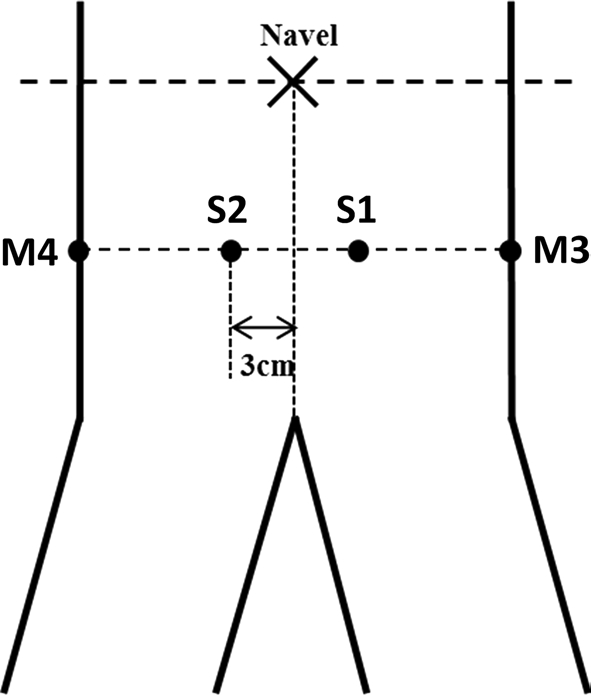
\includegraphics[height=0.20\textheight]{figuras/li2019/posicion-electrodos.png}
    \caption{Ubicación de los electrodos de inyección $S1$--$S2$ y de medición $M3$--$M4$ empleada
    en el estudio experimental. Reproducida de Li et al. \cite{li2019electrode}, bajo licencia
    CC BY 4.0.}
    \label{fig:electrodos_li2019}
\end{figure}

Esta configuración constituye un punto de partida y no una ubicación universal, ya que el espesor
adiposo, la geometría pélvica y la posición de la vejiga modifican la distribución de corriente. Su
aplicación en el prototipo requiere evaluar repetibilidad y sensibilidad entre distintos sujetos
\cite{li2019electrode}.

\clearpage

\subsection{Modelos predictivos}



\section{Metodología}

\subsection{Diseño general del sistema}

Se desarrolló un prototipo para medir de forma no invasiva las variaciones de impedancia eléctrica
en la región abdominal asociadas con el llenado vesical. El sistema emplea una configuración
tetrapolar: dos electrodos aplican una corriente alterna y otros dos registran la tensión resultante.
A partir de ambas magnitudes se estima la impedancia del tejido comprendido en la zona de medición.

El dispositivo se organizó en cuatro bloques funcionales. El primero genera una señal sinusoidal de
excitación de 50~kHz; el segundo la convierte en una corriente de amplitud controlada para aplicarla mediante los
electrodos de inyección; el tercero amplifica, filtra y demodula la tensión obtenida por los electrodos
de medición; y el cuarto digitaliza y procesa la señal mediante un microcontrolador ESP32-C3. Los
resultados se transmiten de forma inalámbrica a una interfaz gráfica para su visualización y registro.

\begin{figure}[htbp]
    \centering
    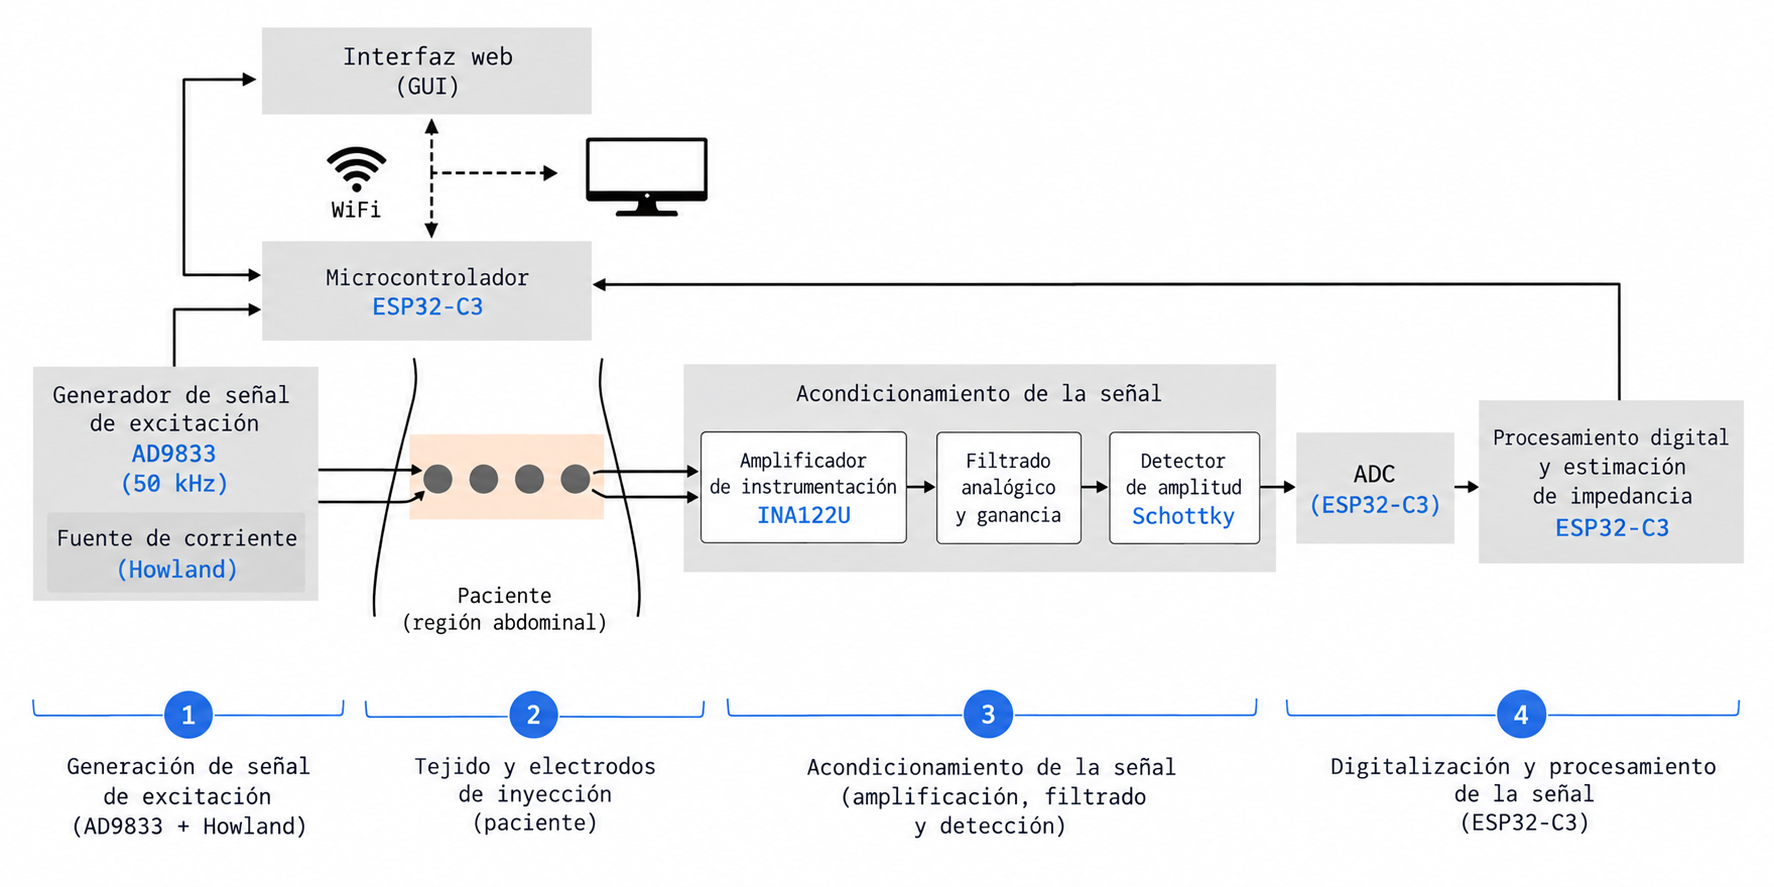
\includegraphics[width=\textwidth]{Diagrama de bloques.png}
    \caption{Diagrama de bloques del sistema de medición de bioimpedancia. El ESP32-C3 configura
    la excitación, digitaliza la señal detectada y transmite los resultados a la interfaz gráfica.}
    \label{fig:diagrama_bloques_sistema}
\end{figure}

\subsection{Diseño del circuito de medición}

El circuito electrónico fue diseñado en KiCad e integrado en una placa de circuito impreso (PCB). Para
facilitar su análisis, se dividió en las etapas de generación de la excitación, inyección de corriente,
adquisición de tensión y control digital.

\subsubsection{Generación de la señal de excitación}

La señal de excitación se generó mediante un módulo AD9833, configurado y alimentado por el microcontrolador
ESP32-C3. El generador se programó para producir una onda sinusoidal de
50~kHz y aproximadamente 0,6~V pico a pico.

La salida del AD9833 presentaba una componente continua, por lo que se incorporó una etapa de
acoplamiento en alterna formada por un capacitor de 10~$\mu$F en serie y una resistencia de 500~$\Omega$
conectada a la referencia del circuito. Ambos componentes forman un filtro pasaaltos de primer orden,
cuya frecuencia de corte se calcula como

\begin{equation}
    f_c=\frac{1}{2\pi RC}
    =\frac{1}{2\pi(500~\Omega)(10~\mu\mathrm{F})}
    \approx 31{,}8~\mathrm{Hz}.
\end{equation}

Como la frecuencia de excitación de 50~kHz es muy superior a la frecuencia de corte, la etapa elimina
la componente continua sin atenuar de manera significativa la señal sinusoidal de interés.

\subsubsection{Inyección de corriente}

Para acondicionar la señal antes de la fuente de corriente se utilizó una sección del TL082 en
configuración inversora. Con una resistencia de entrada de 1~k$\Omega$ y una resistencia de
realimentación de 10~k$\Omega$, se midió a la salida una amplitud de
3,22~V pico a pico.

La segunda sección del TL082 se utilizó para implementar una
fuente de corriente Howland. Esta topología se emplea en sistemas de bioimpedancia debido a que puede
proporcionar una corriente estable sobre un intervalo de cargas y frecuencias, aunque su desempeño
depende del ancho de banda del amplificador y del apareamiento de las resistencias
\cite{nwokoye2024howland}. La configuración implementada se muestra en la
Figura~\ref{fig:howland}.

\begin{figure}[htbp]
    \centering
    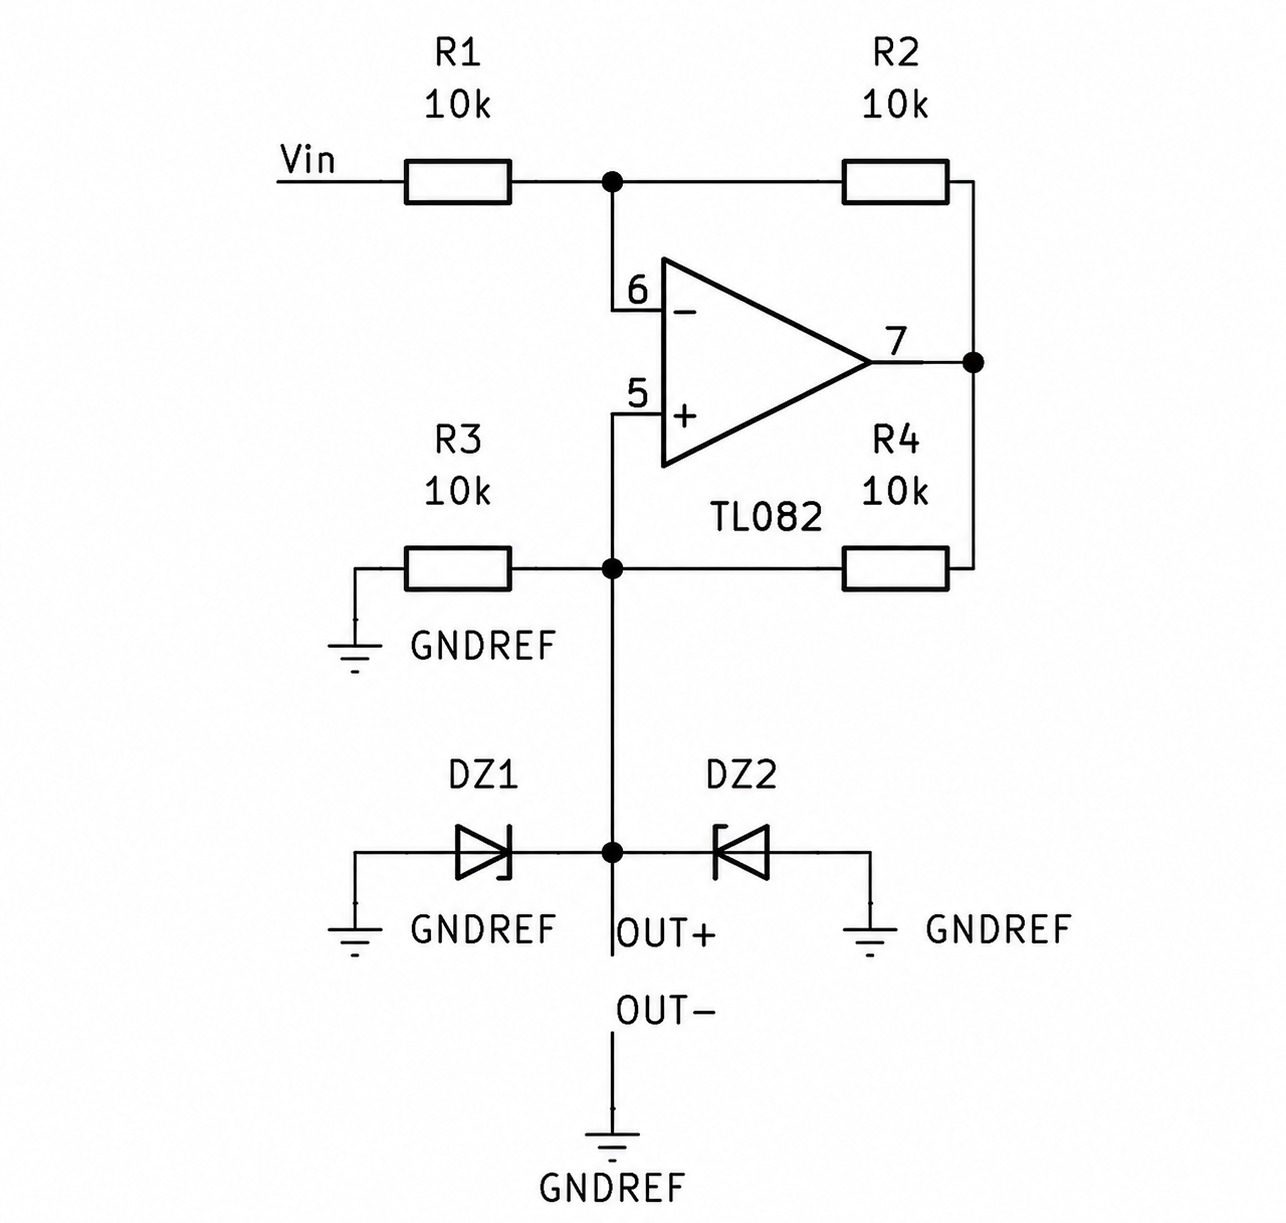
\includegraphics[width=0.66\textwidth]{figuras/howland.png}
    \caption{Esquema de la fuente de corriente Howland implementada. Las cuatro resistencias son de
    10~k$\Omega$ y los diodos Zener de protección están conectados en antiparalelo entre los
    terminales de salida.}
    \label{fig:howland}
\end{figure}

Para que la fuente se encuentre balanceada, las resistencias deben satisfacer la condición

\begin{equation}
    R_1R_4=R_2R_3.
\end{equation}

En el circuito implementado se seleccionaron cuatro resistencias iguales de 10~k$\Omega$, con lo que se
cumple esta relación. En estas condiciones, la corriente de salida queda determinada por la
tensión aplicada a la fuente y una de las resistencias de 10~k$\Omega$:

\begin{equation}
    I_{\mathrm{out}}=\frac{V_{\mathrm{in}}}{R_1}.
\end{equation}

En el cálculo, $V_{\mathrm{in}}$ corresponde a la tensión medida a la entrada de la fuente de Howland,
es decir, a la salida de la etapa inversora descripta anteriormente (3,22~V pico a pico).
Con $R_1=10~\mathrm{k}\Omega$, esto da una corriente nominal de inyección de

\begin{equation}
    I_{\mathrm{out}}\approx\frac{3{,}22~\mathrm{V}}{10~\mathrm{k}\Omega}
    =322~\mu\mathrm{A}_{\mathrm{pp}}\approx 114~\mu\mathrm{A}_{\mathrm{rms}}.
\end{equation}

Este es un valor teórico de diseño, calculado a partir de la relación tensión--corriente del circuito de
Howland y no de una medición directa. Debido a que la amplitud real entregada por el AD9833, la ganancia
efectiva de la etapa inversora y el apareamiento real de las resistencias del Howland pueden diferir de
sus valores nominales, la corriente efectivamente entregada al paciente debe determinarse
experimentalmente aplicando la fuente sobre una resistencia de carga conocida y midiendo la tensión
resultante. Además, la verificación de seguridad debe realizarse con el procedimiento y las magnitudes
establecidos por IEC~60601-1, considerando la frecuencia de 50~kHz y la clasificación de la parte
aplicada \cite{iec60601}.

\subsubsection{Adquisición y acondicionamiento de la tensión}

La tensión diferencial captada por los electrodos de medición ingresa al amplificador de
instrumentación INA122U. Su salida se acondiciona mediante seis etapas con amplificadores TL082 y
TL084, antes de aplicarse al detector Schottky y al conversor analógico--digital. El diseño busca
preservar la componente de 50~kHz y obtener una amplitud suficiente para la detección.

El acondicionamiento combina amplificación y filtrado pasaaltos y pasabajos. Los componentes se seleccionaron a fin 
de conservar la señal de interés y reducir el ruido fuera de la banda de frecuencia estudiada. La etapa final 
incluye un detector de envolvente y un filtro pasabajos para obtener una señal de salida continua proporcional a 
la amplitud de la señal de 50~kHz. A continuación se describen la configuración
de cada etapa y su respuesta calculada. Las Figuras~\ref{fig:acq_inicial} a~\ref{fig:acq_detector}
permiten seguir el recorrido de la señal por bloques. El esquema completo se incluye en el
Anexo~\ref{anexo:esquema_circuito}.

\paragraph{Instrumentación y amplificación inicial.}
El INA122U es un amplificador de instrumentación que amplifica la diferencia de potencial entre los
electrodos de medición y rechaza la componente de modo común presente en ambas entradas. Su estructura
interna utiliza dos amplificadores operacionales y una red de resistencias. La ganancia se ajusta
mediante una resistencia externa $R_g$ según
la relación \cite{ti_ina122}
\begin{equation}
    G_{\mathrm{INA}}=5+\frac{200~\mathrm{k}\Omega}{R_g},\qquad
    \lim_{R_g\to\infty}G_{\mathrm{INA}}=5.
\end{equation}

La estructura interna del INA122 y la conexión de la resistencia externa de ganancia se muestran en la
Figura~\ref{fig:ina_estructura}.

\begin{figure}[htbp]
    \centering
    \includegraphics[page=12,trim=235 515 235 140,clip,width=0.42\textwidth]{Informe final GRUPO2 Chidori (1).pdf}
    \caption{Estructura interna del INA122 y conexión de la resistencia externa de ganancia.
    En el diseño se dejan abiertos los terminales de dicha resistencia para obtener una ganancia
    nominal de 5. Esquema de Texas Instruments \cite{ti_ina122}.}
    \label{fig:ina_estructura}
\end{figure}

En este diseño no se coloca una resistencia externa de ganancia, por lo que se adopta el valor mínimo
de 5. Esta elección permite conservar un mayor ancho de banda que el disponible con ganancias más
elevadas y distribuir la amplificación restante entre las etapas de acondicionamiento. Para esta
ganancia, el ancho de banda típico considerado es del orden de 100~kHz, por encima de la frecuencia
de excitación de 50~kHz, aunque su respuesta no es completamente plana a esa frecuencia
\cite{ti_ina122}. Esta respuesta se ilustra en la Figura~\ref{fig:respuesta_frecuencia_ina122}.

\begin{figure}[htbp]
    \centering
    \includegraphics[page=12,trim=150 150 160 480,clip,width=0.62\textwidth]{Informe final GRUPO2 Chidori (1).pdf}
    \caption{Respuesta en frecuencia del INA122 para distintos valores de ganancia. Para $G=5$,
    la frecuencia de corte se encuentra aproximadamente en 100~kHz, mientras que a 50~kHz la
    ganancia ya presenta una atenuación respecto de su valor de baja frecuencia. Adaptada de
    Texas Instruments \cite{ti_ina122}.}
    \label{fig:respuesta_frecuencia_ina122}
\end{figure}

\paragraph{Funciones de transferencia y ganancia.}
Para describir cómo cada etapa modifica la señal se utiliza su función de transferencia
$H_i(s)$, definida como la relación entre las transformadas de Laplace de las tensiones de salida
y entrada, con condiciones iniciales nulas:
\begin{equation}
    H_i(s)=\frac{V_{\mathrm{sal},i}(s)}{V_{\mathrm{ent},i}(s)}.
\end{equation}
El subíndice $i$ identifica las seis etapas posteriores al amplificador de instrumentación, en el
orden en que las atraviesa la señal: seguidor inicial ($H_1$), amplificador inversor ($H_2$),
primer acoplamiento pasaaltos y filtro inversor ($H_3$), pasaaltos activo ($H_4$), pasabajos pasivo
con seguidor ($H_5$) y amplificador final ($H_6$). Cada función incluye los componentes pasivos
asociados a esa etapa.

En régimen sinusoidal permanente se evalúa $s=j2\pi f$, donde $f$ es la frecuencia y $j$ la unidad
imaginaria. La magnitud $|H_i(j2\pi f)|$ expresa la ganancia de amplitud, es decir, el cociente entre
las amplitudes de salida y entrada a esa frecuencia; el argumento de $H_i$ representa el desfase.
Una magnitud mayor que uno indica amplificación, menor que uno indica atenuación e igual a uno
indica conservación de la amplitud. Para señales sinusoidales sin recorte, este cociente puede
calcularse con valores de pico, pico a pico o eficaces, siempre que se use la misma magnitud en
entrada y salida. Las ganancias se expresan en V/V y se evalúan a 50~kHz para caracterizar la
respuesta a la señal de excitación. En una etapa resistiva inversora, el signo negativo de la
transferencia indica inversión de polaridad, mientras que su valor absoluto determina cuánto
se amplifica la amplitud.

\paragraph{Seguidor de tensión y amplificación inicial.}
En la Figura~\ref{fig:acq_inicial}, R1 y R2 corresponden a las resistencias de entrada y realimentación de U5B, respectivamente.

\begin{figure}[htbp]
    \centering
    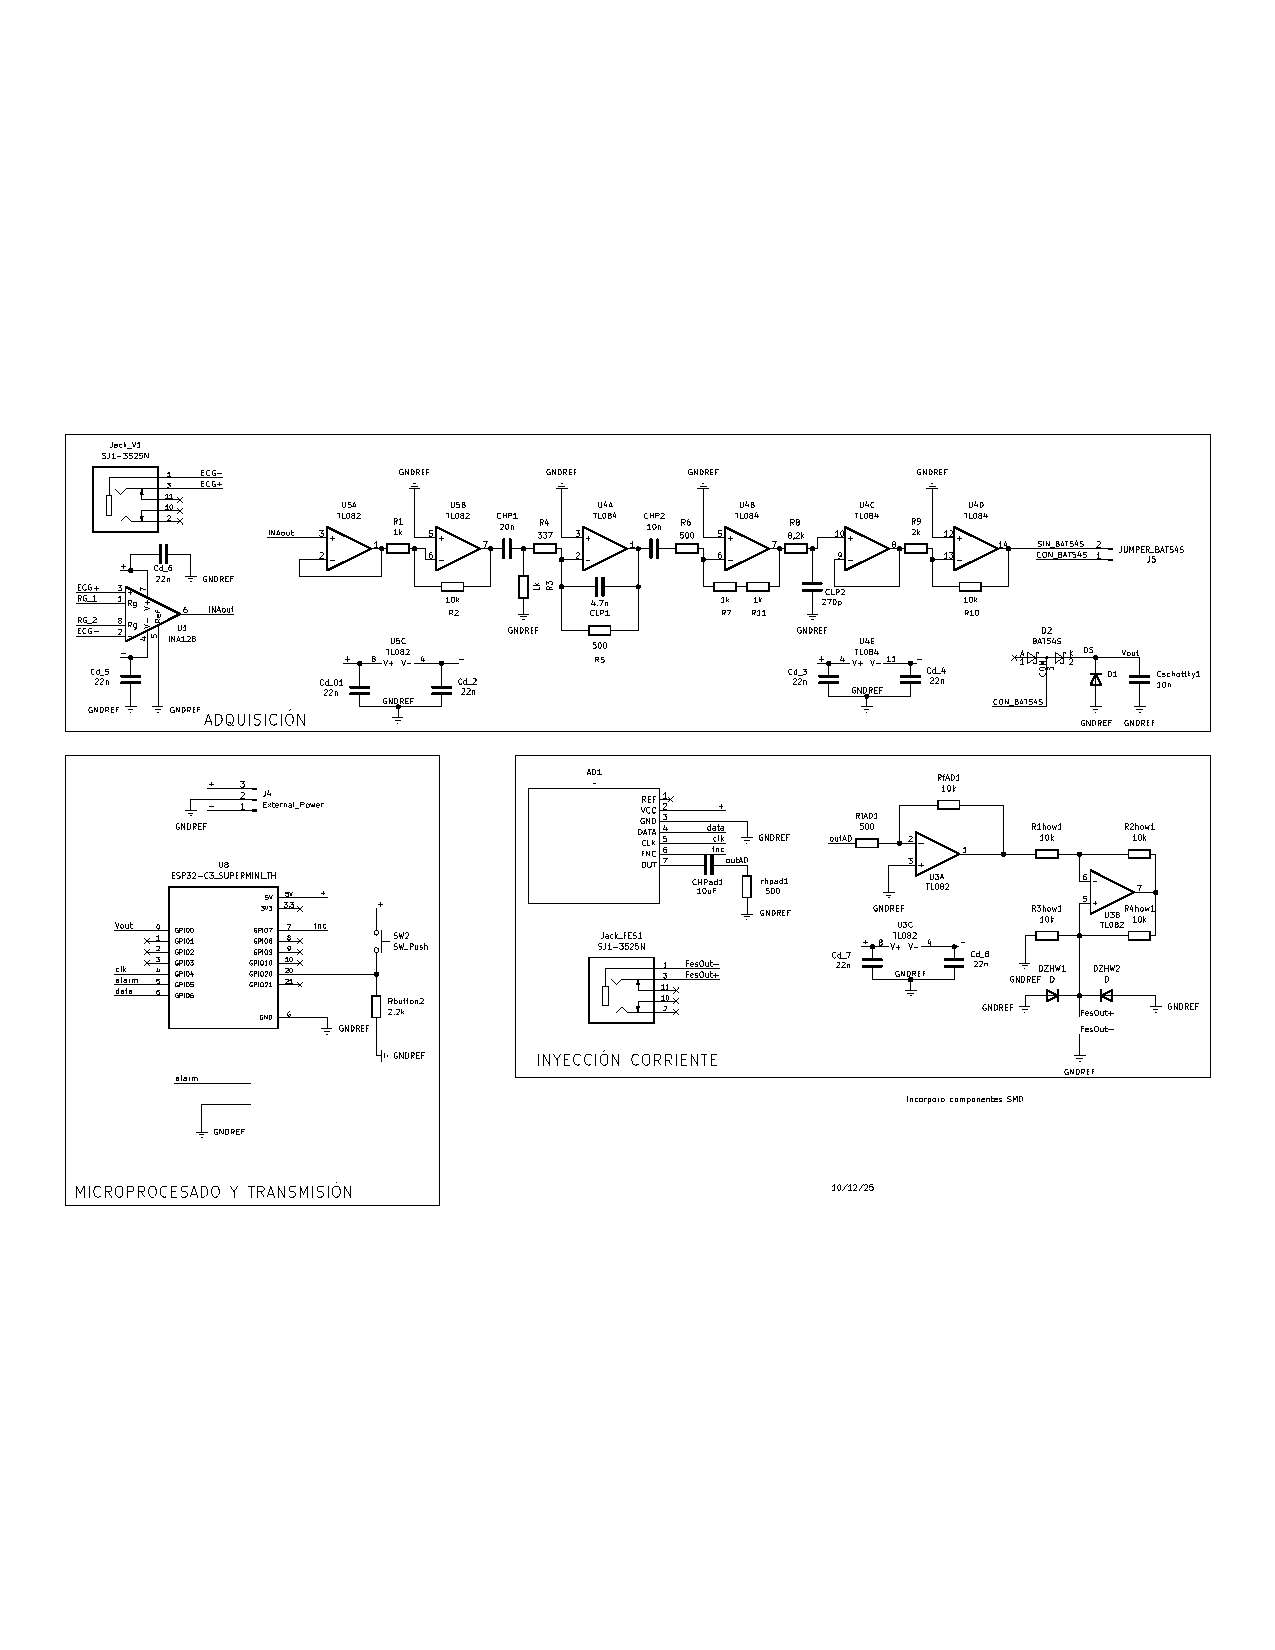
\includegraphics[page=1,viewport=125.87 492.11 236.17 569.08,clip,width=0.55\textwidth]{figuras/esquema_circuito.pdf}
    \caption{Seguidor U5A y amplificador inversor U5B, desde la entrada INAout.}
    \label{fig:acq_inicial}
\end{figure}


La primera etapa se conecta como seguidor de tensión: conserva aproximadamente la amplitud y desacopla al INA122U
de la carga de la etapa siguiente. La segunda etapa es un amplificador inversor con una resistencia
de entrada de 1~k$\Omega$ y una resistencia de realimentación de 10~k$\Omega$. En las ecuaciones,
$R_{\mathrm{in}}$ y $R_f$ representan las resistencias de entrada y realimentación de la etapa
considerada, respectivamente. Para operacionales ideales, las dos primeras etapas tienen las transferencias
\begin{equation}
    H_1=1,\qquad H_2=-\frac{R_f}{R_{\mathrm{in}}}=-10.
\end{equation}
Para el cálculo de las amplitudes ideales se adopta una señal de referencia de 12~mV pico a pico
a la salida del amplificador de instrumentación. Con esta entrada, la segunda etapa entrega
idealmente 120~mV pico a pico. Las mediciones del prototipo se presentan por separado en resultados.

\paragraph{Primer pasaaltos y filtro inversor.}
La Figura~\ref{fig:acq_filtro1} muestra el bloque entre las salidas de U5B y U4A. En las expresiones siguientes, $R_m$ corresponde a R3, $R_{\mathrm{in}}$ a R4, $R_f$ a R5, $C_a$ a CHP1 y $C_f$ a CLP1.

\begin{figure}[htbp]
    \centering
    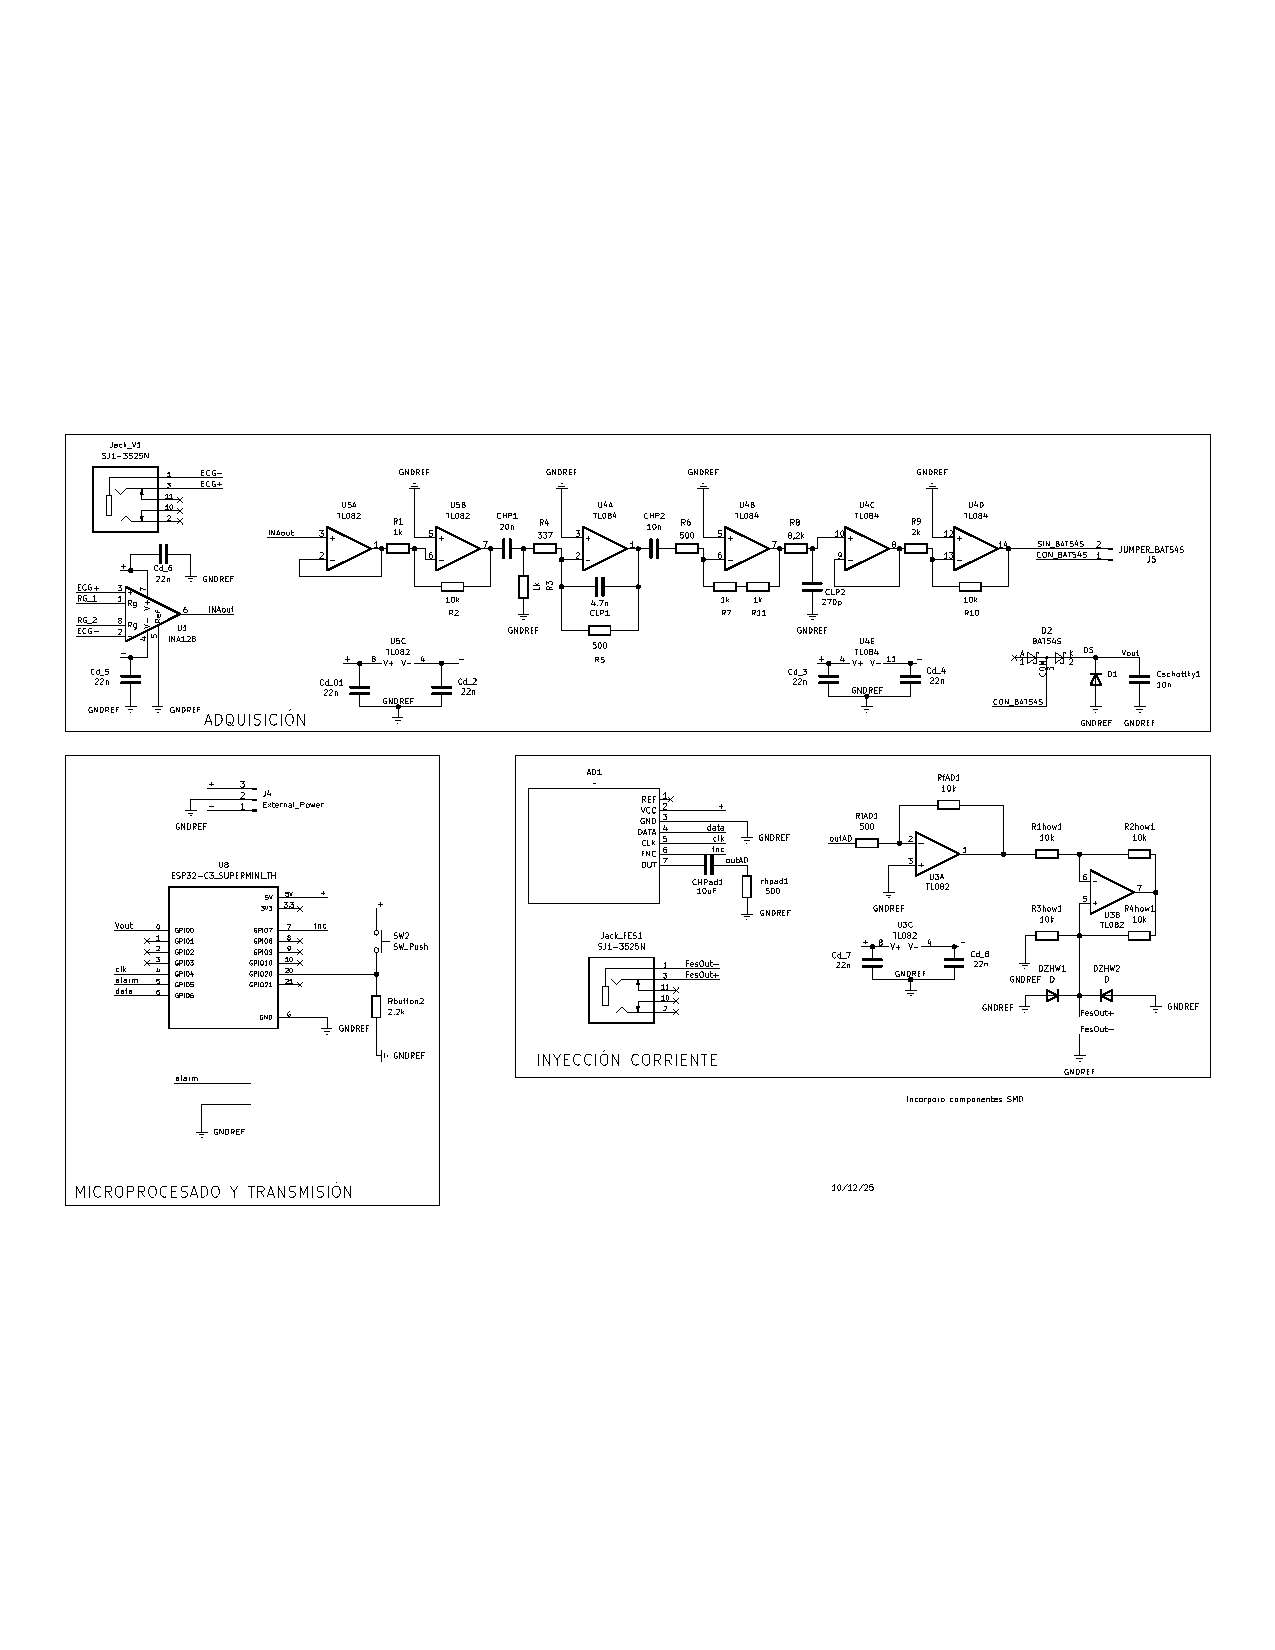
\includegraphics[page=1,viewport=237.06 472.09 307.33 569.53,clip,width=0.37\textwidth]{figuras/esquema_circuito.pdf}
    \caption{Primer acoplamiento pasaaltos y filtro inversor U4A.}
    \label{fig:acq_filtro1}
\end{figure}


La salida de la segunda etapa se acopla mediante un capacitor de 20~nF a un nodo conectado a masa
a través de una resistencia de 1~k$\Omega$. Desde ese nodo, una resistencia de entrada de
337~$\Omega$ conduce a la entrada inversora del tercer operacional. Esta última resistencia carga
el pasaaltos, porque su extremo inversor se encuentra a masa virtual en el modelo ideal.
Denominando $R_m$ a la resistencia de 1~k$\Omega$ conectada a masa y $C_a$ al capacitor
de acoplamiento de 20~nF, se obtiene
\begin{equation}
    R_p=R_m\parallel R_{\mathrm{in}}
    =\frac{1000\times337}{1000+337}~\Omega\approx252{,}1~\Omega,
\end{equation}
\begin{equation}
    f_{\mathrm{HP1}}=\frac{1}{2\pi R_pC_a}
    \approx31{,}6~\mathrm{kHz}.
    \label{eq:fc1}
\end{equation}
Con el capacitor de 20~nF, la frecuencia de corte es aproximadamente 32~kHz al considerar la carga de
la etapa siguiente. El cálculo con la resistencia a masa solamente no representa la red conectada.

La tercera etapa utiliza una resistencia de realimentación de 500~$\Omega$ en paralelo con un
capacitor de 4,7~nF, que introduce un polo pasabajos. Se denomina $C_a$ al capacitor de acoplamiento
de 20~nF y $C_f$ al capacitor de realimentación de 4,7~nF. Con $s=j2\pi f$,
\begin{equation}
    Z_f(s)=\frac{R_f}{1+sR_fC_f},\qquad
    f_{\mathrm{LP1}}=\frac{1}{2\pi R_fC_f}\approx67{,}7~\mathrm{kHz}.
\end{equation}
Desde la entrada del capacitor de acoplamiento hasta la salida de la tercera etapa, la transferencia
ideal conjunta es
\begin{equation}
    H_3(s)=-\frac{R_f}{R_{\mathrm{in}}}
    \frac{sR_pC_a}
    {(1+sR_pC_a)(1+sR_fC_f)}.
\end{equation}
A 50~kHz su magnitud es aproximadamente 1,01: la amplificación de la tercera etapa compensa prácticamente la
atenuación de las redes de filtrado a esa frecuencia. Los cortes de 31,6 y 67,7~kHz pertenecen a las
redes individuales; los límites de esta sección completa a $-3$~dB respecto de su máximo son
aproximadamente 18,2 y 117,5~kHz, con máximo a 46,2~kHz.

\paragraph{Segundo pasaaltos activo.}
En la Figura~\ref{fig:acq_filtro2}, $C_a$ corresponde a CHP2, $R_{\mathrm{in}}$ a R6 y $R_f$ a la suma de R7 y R11.

\begin{figure}[htbp]
    \centering
    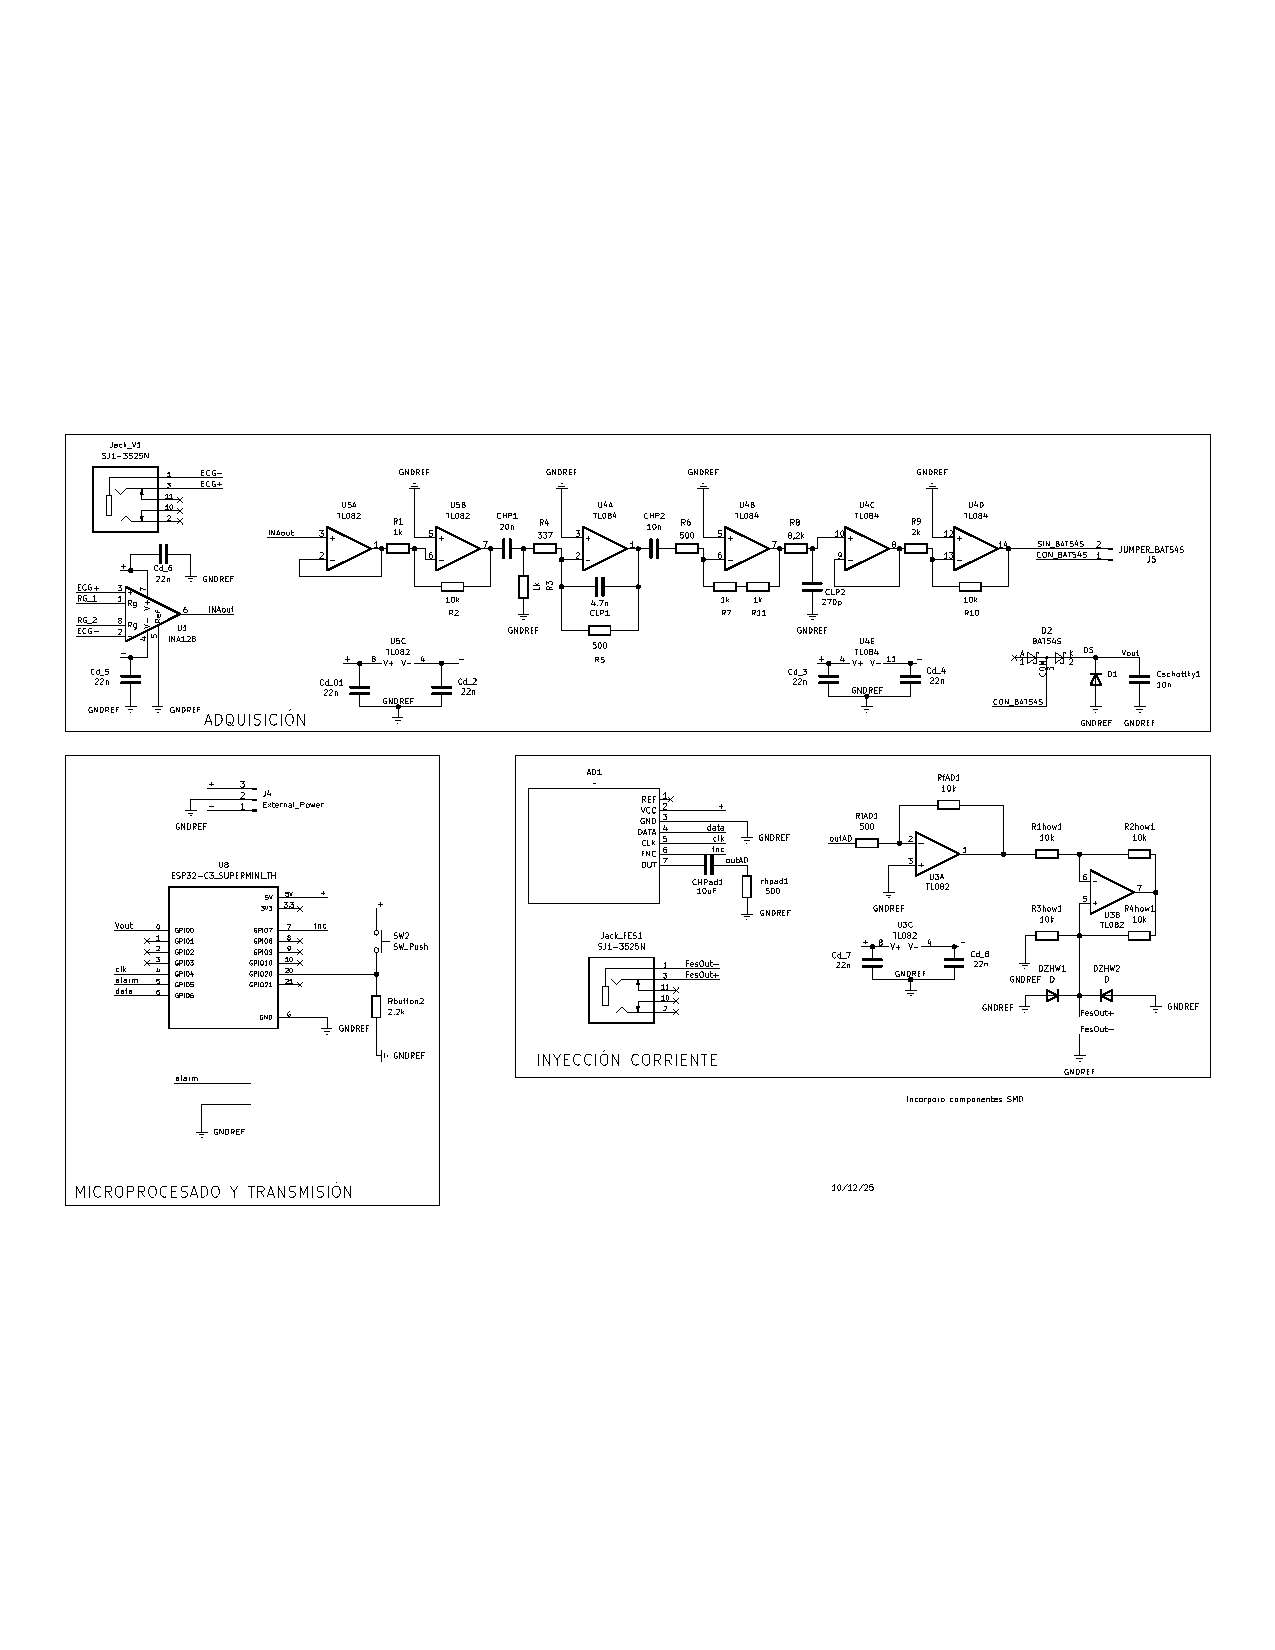
\includegraphics[page=1,viewport=308.22 491.66 374.94 569.53,clip,width=0.35\textwidth]{figuras/esquema_circuito.pdf}
    \caption{Segundo pasaaltos activo con U4B; R7 y R11 forman la realimentación.}
    \label{fig:acq_filtro2}
\end{figure}


La cuarta etapa es un amplificador inversor cuya entrada contiene un capacitor de 10~nF en serie
con una resistencia de 500~$\Omega$. La realimentación está formada por dos resistencias de
1~k$\Omega$ en serie, equivalentes a 2~k$\Omega$. Denominando $C_a$ al capacitor de entrada
de esta etapa, su transferencia y frecuencia de corte ideales son
\begin{equation}
    H_4(s)=-\frac{R_f}{R_{\mathrm{in}}+1/(sC_a)},\qquad
    f_{\mathrm{HP2}}=\frac{1}{2\pi R_{\mathrm{in}}C_a}\approx31{,}8~\mathrm{kHz}.
\end{equation}
Con el capacitor de 10~nF y la resistencia de entrada de 500~$\Omega$, la frecuencia de corte
es 31,8~kHz, inferior a la frecuencia de excitación de 50~kHz. A esta frecuencia, la ganancia
de amplitud es $|H_4|\approx3{,}374$; en el modelo ideal, se aproxima a 4 para frecuencias
mucho mayores que la de corte.

\paragraph{Pasabajos, seguidor y amplificación final.}
La Figura~\ref{fig:acq_final} reúne las dos últimas etapas. En el filtro, $R$ corresponde a R8 y $C$ a CLP2; en el amplificador final, las resistencias de entrada y realimentación son R9 y R10.

\begin{figure}[htbp]
    \centering
    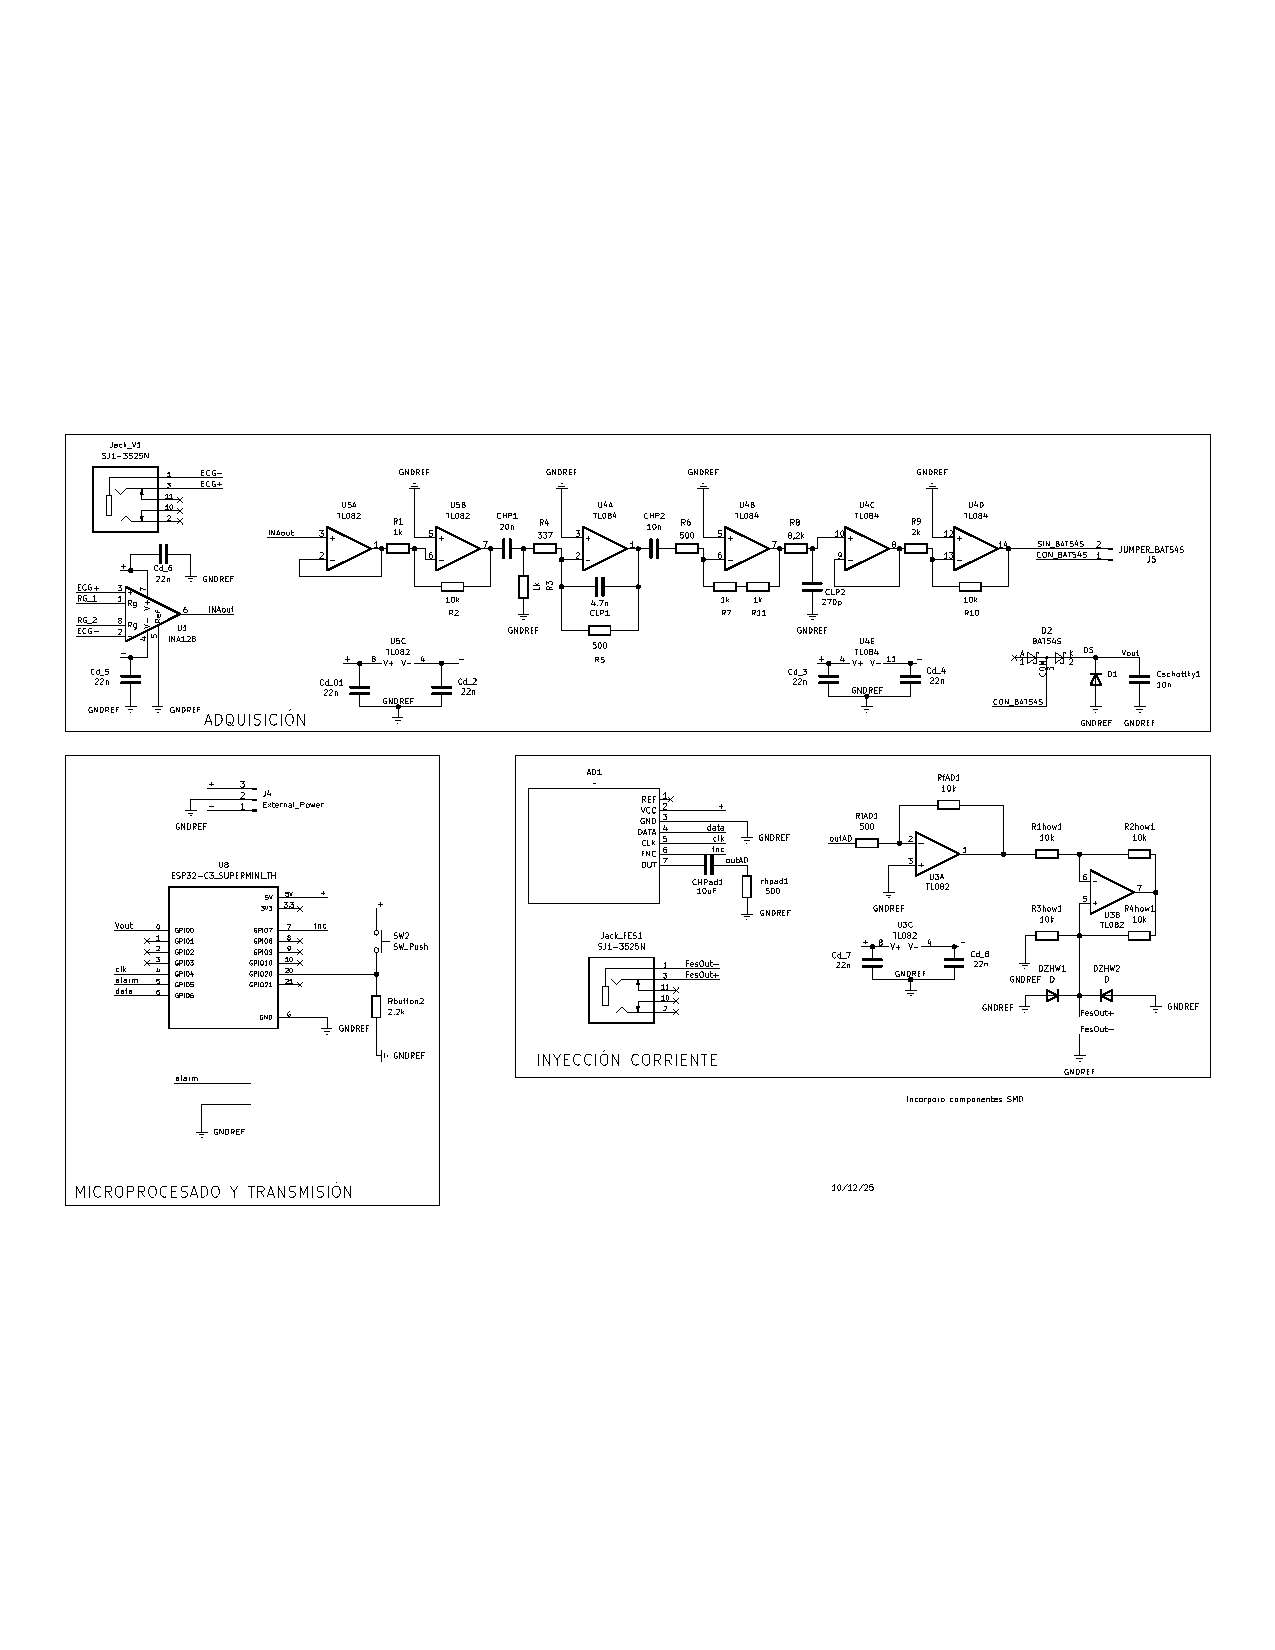
\includegraphics[page=1,viewport=375.83 491.66 486.13 569.53,clip,width=0.55\textwidth]{figuras/esquema_circuito.pdf}
    \caption{Pasabajos R8--CLP2, seguidor U4C y amplificador inversor U4D.
    El valor de R9 utilizado es 2,2~k$\Omega$; el rótulo de 2~k$\Omega$ del esquema no corresponde al valor montado.}
    \label{fig:acq_final}
\end{figure}


A continuación se dispone un pasabajos pasivo con una resistencia $R$ de 8,2~k$\Omega$ en serie
y un capacitor $C$ de 270~pF a masa. El quinto operacional se conecta como seguidor después del
filtro para desacoplarlo de la carga del amplificador final. La transferencia ideal de esta sección es
\begin{equation}
    H_5(s)=\frac{1}{1+sRC},\qquad
    f_{\mathrm{LP2}}=\frac{1}{2\pi RC}\approx71{,}9~\mathrm{kHz}.
\end{equation}
A 50~kHz, $|H_5|\approx0{,}821$.

La sexta y última etapa es un amplificador inversor con una resistencia de entrada de 2,2~k$\Omega$
y una resistencia de realimentación de 10~k$\Omega$:
\begin{equation}
    H_6=-\frac{R_f}{R_{\mathrm{in}}}=-\frac{10}{2{,}2}\approx-4{,}545.
\end{equation}
Esta ganancia se seleccionó considerando la amplitud entregada por las etapas de filtrado.
Permite obtener una señal del orden de 1,52~V pico a pico antes del detector a partir del
punto de funcionamiento adoptado de 12~mV pico a pico en la salida del amplificador de instrumentación.

\begin{table}[htbp]
    \centering
    \caption{Ganancias ideales de las etapas de acondicionamiento a 50~kHz desde la salida del INA122U.}
    \label{tab:cadena_acondicionamiento}
    \begin{tabular}{lll}
        \hline
        Etapa & Función & Magnitud de ganancia \\
        \hline
        Primera & Seguidor & 1 \\
        Segunda & Inversor & 10 \\
        Tercera & Acoplamiento cargado y filtro inversor & 1,01 \\
        Cuarta & Pasaaltos activo & 3,374 \\
        Quinta & Pasabajos y seguidor & 0,821 \\
        Sexta & Inversor & 4,545 \\
        \hline
    \end{tabular}
\end{table}

\paragraph{Ganancia y banda de la cadena.}
La transferencia posterior al INA es $H_{\mathrm{ac}}(s)=\prod_{i=1}^{6}H_i(s)$.
Calculando con los valores sin redondear se obtiene
\begin{equation}
    |H_{\mathrm{ac}}(50~\mathrm{kHz})|\approx127{,}1.
\end{equation}
Si se incluye un INA ideal con ganancia 5, el producto es aproximadamente 635,4. Para dimensionar
la salida a partir de los 12~mV pico a pico adoptados como referencia a la salida del amplificador
de instrumentación, se utiliza solamente la ganancia posterior al INA; no corresponde
multiplicar esa amplitud nuevamente por 5.

\paragraph{Respuesta en frecuencia ideal.}
La Figura~\ref{fig:bode_cadena} muestra el diagrama de Bode de magnitud calculado a partir
de las seis transferencias ideales, desde la salida del INA hasta la salida del último
amplificador, antes del detector. La ganancia a 50~kHz es aproximadamente 127,1~V/V
(42,1~dB). Los límites de banda a $-3$~dB respecto del máximo son aproximadamente
24,6 y 89,9~kHz, con un ancho de banda de 65,3~kHz. La frecuencia de excitación de
50~kHz queda dentro de esta banda.

\begin{figure}[htbp]
    \centering
    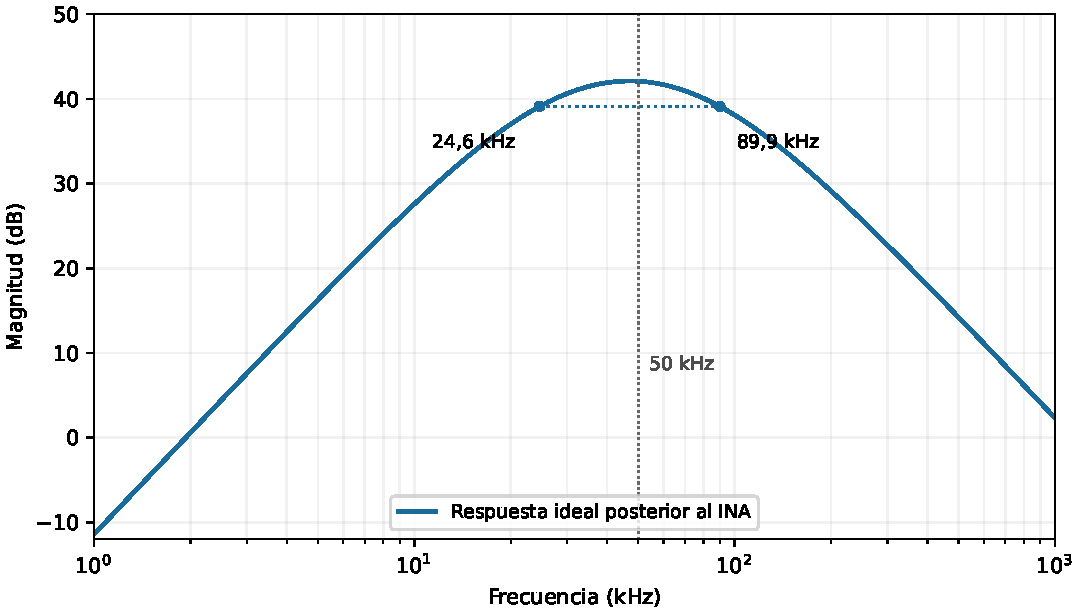
\includegraphics[width=0.92\textwidth]{figuras/bode_cadena.pdf}
    \caption{Diagrama de Bode de magnitud ideal de las seis etapas posteriores al INA,
    calculado como $20\log_{10}|H_{\mathrm{ac}}|$. Se indican la frecuencia de excitación
    de 50~kHz y los límites de banda a aproximadamente $-3$~dB respecto del máximo.
    La curva corresponde al cálculo teórico, no a mediciones experimentales.}
    \label{fig:bode_cadena}
\end{figure}

Los límites de banda de la cadena se obtienen del producto de las transferencias y no
coinciden con los cortes de los filtros considerados por separado. Estos cálculos emplean
los valores nominales de los componentes y operacionales ideales; la respuesta medida
del circuito se contrastará con esta referencia en la sección de resultados.

\paragraph{Amplitudes previstas y verificación.}
El circuito se alimenta con dos baterías de 3,7~V en serie, cuyo punto medio se toma como referencia de masa,
proporcionando una alimentación simétrica de $\pm3{,}7$~V, verificados en el conector de alimentación.
La Tabla~\ref{tab:amplitudes_propuestas} presenta las amplitudes calculadas usando 12~mV pico a pico
en la salida del amplificador de instrumentación y las ganancias ideales de cada etapa.
\begin{table}[htbp]
    \centering
    \caption{Amplitudes calculadas a 50~kHz para una entrada de 12~mV pico a pico desde el amplificador de instrumentación.}
    \label{tab:amplitudes_propuestas}
    \begin{tabular}{lr}
        \hline
        Punto & Tensión pico a pico (mV) \\
        \hline
        Salida del amplificador de instrumentación & 12 \\
        Salida del primer seguidor & 12 \\
        Salida del amplificador de ganancia diez & 120 \\
        Salida del primer filtro inversor & 121 \\
        Salida del pasaaltos activo & 409 \\
        Salida del segundo seguidor & 335 \\
        Salida del amplificador final, antes del detector & 1525 \\
        \hline
    \end{tabular}
\end{table}
La salida final prevista de 1,52~V pico a pico corresponde a una amplitud de aproximadamente
0,76~V de pico para una senoide. En la sección de resultados se comparará esta estimación con la señal medida en el prototipo.

\paragraph{Detección y salida hacia el conversor.}
La Figura~\ref{fig:acq_detector} muestra el conector J5 y el circuito detector.
El esquema distingue las conexiones SIN\_BAT54S y CON\_BAT54S. El bloque incluye
D2 (BAT54S), el diodo D1 y el capacitor Cschottky1 de 10~nF.
Este bloque funciona como un detector de envolvente, entregando una tensión continua proporcional a la amplitud de la señal de 50~kHz
y permite su posterior digitalización. 

El BAT54S contiene dos diodos Schottky en serie, con acceso a la unión entre ambos mediante
el pin 3. Su baja caída de tensión directa permite rectificar señales de pequeña amplitud
\cite{nexperia_bat54s}. En la conexión mostrada, la señal ingresa por ese punto intermedio
y se utiliza el diodo comprendido entre los pines 3 y 2, cuyo cátodo se conecta a Vout.
El pin 1 queda sin conexión, por lo que el segundo diodo interno no interviene en la detección.

Durante los máximos positivos de la señal, el diodo conduce cuando la tensión de entrada
supera la tensión almacenada en el capacitor más la caída directa del diodo. En ese intervalo,
circula corriente hacia Cschottky1 y aumenta su tensión. Cuando la entrada disminuye por
debajo de esa condición, el diodo deja de conducir y bloquea la descarga del capacitor hacia
la etapa amplificadora. La carga almacenada mantiene la salida entre máximos sucesivos.
Así, el diodo y el capacitor forman un detector de pico positivo; cuando la amplitud varía
lentamente, su salida permite seguir la envolvente de la señal.

Para una senoide centrada en cero, de amplitud pico a pico $V_{\mathrm{pp}}$, una aproximación
de la tensión detectada es
\begin{equation}
    V_{\mathrm{det}}\approx\frac{V_{\mathrm{pp}}}{2}-V_F,
\end{equation}
donde $V_F$ representa la caída directa durante la conducción. Esta expresión supone que el
capacitor alcanza aproximadamente el pico y que su descarga entre ciclos es pequeña.


\begin{figure}[htbp]
    \centering
    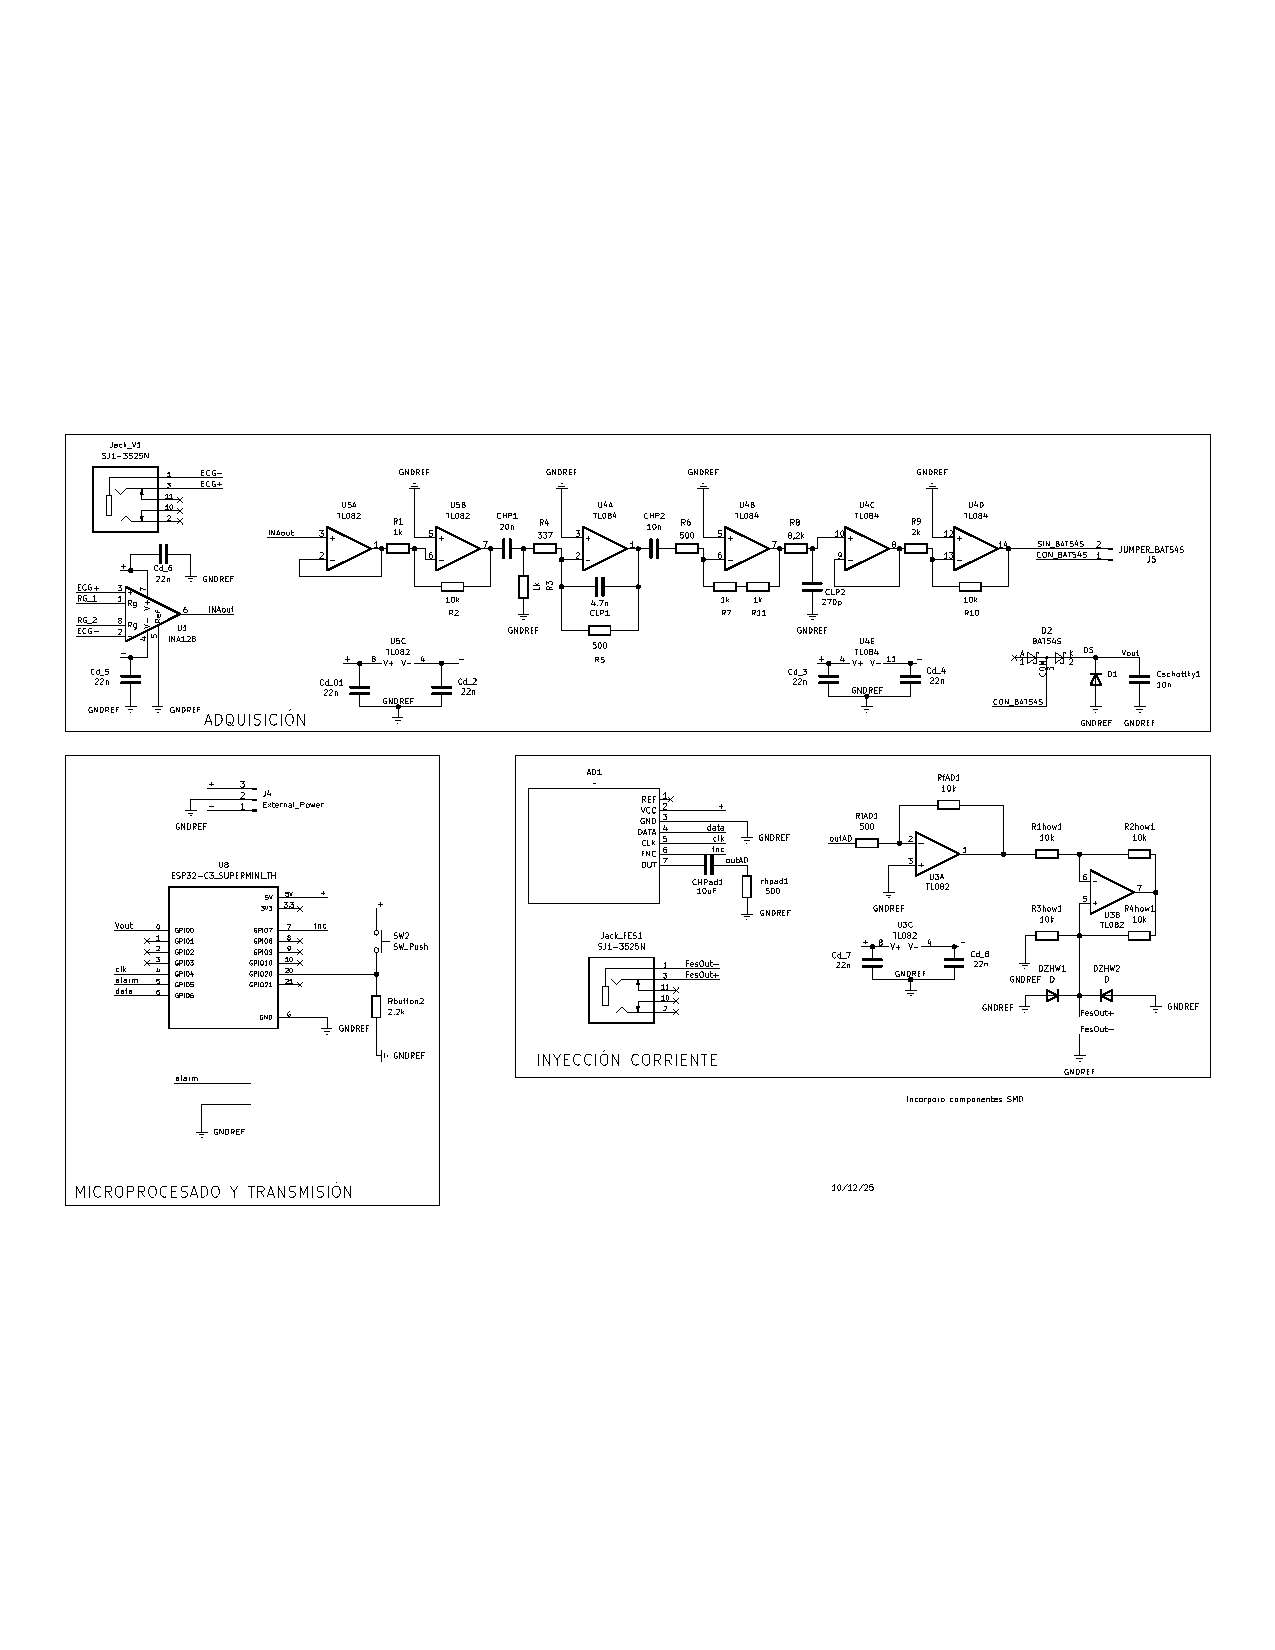
\includegraphics[page=1,viewport=486.58 518.36 577.75 535.27,clip,width=0.43\textwidth]{figuras/esquema_circuito.pdf}
    \par\medskip
    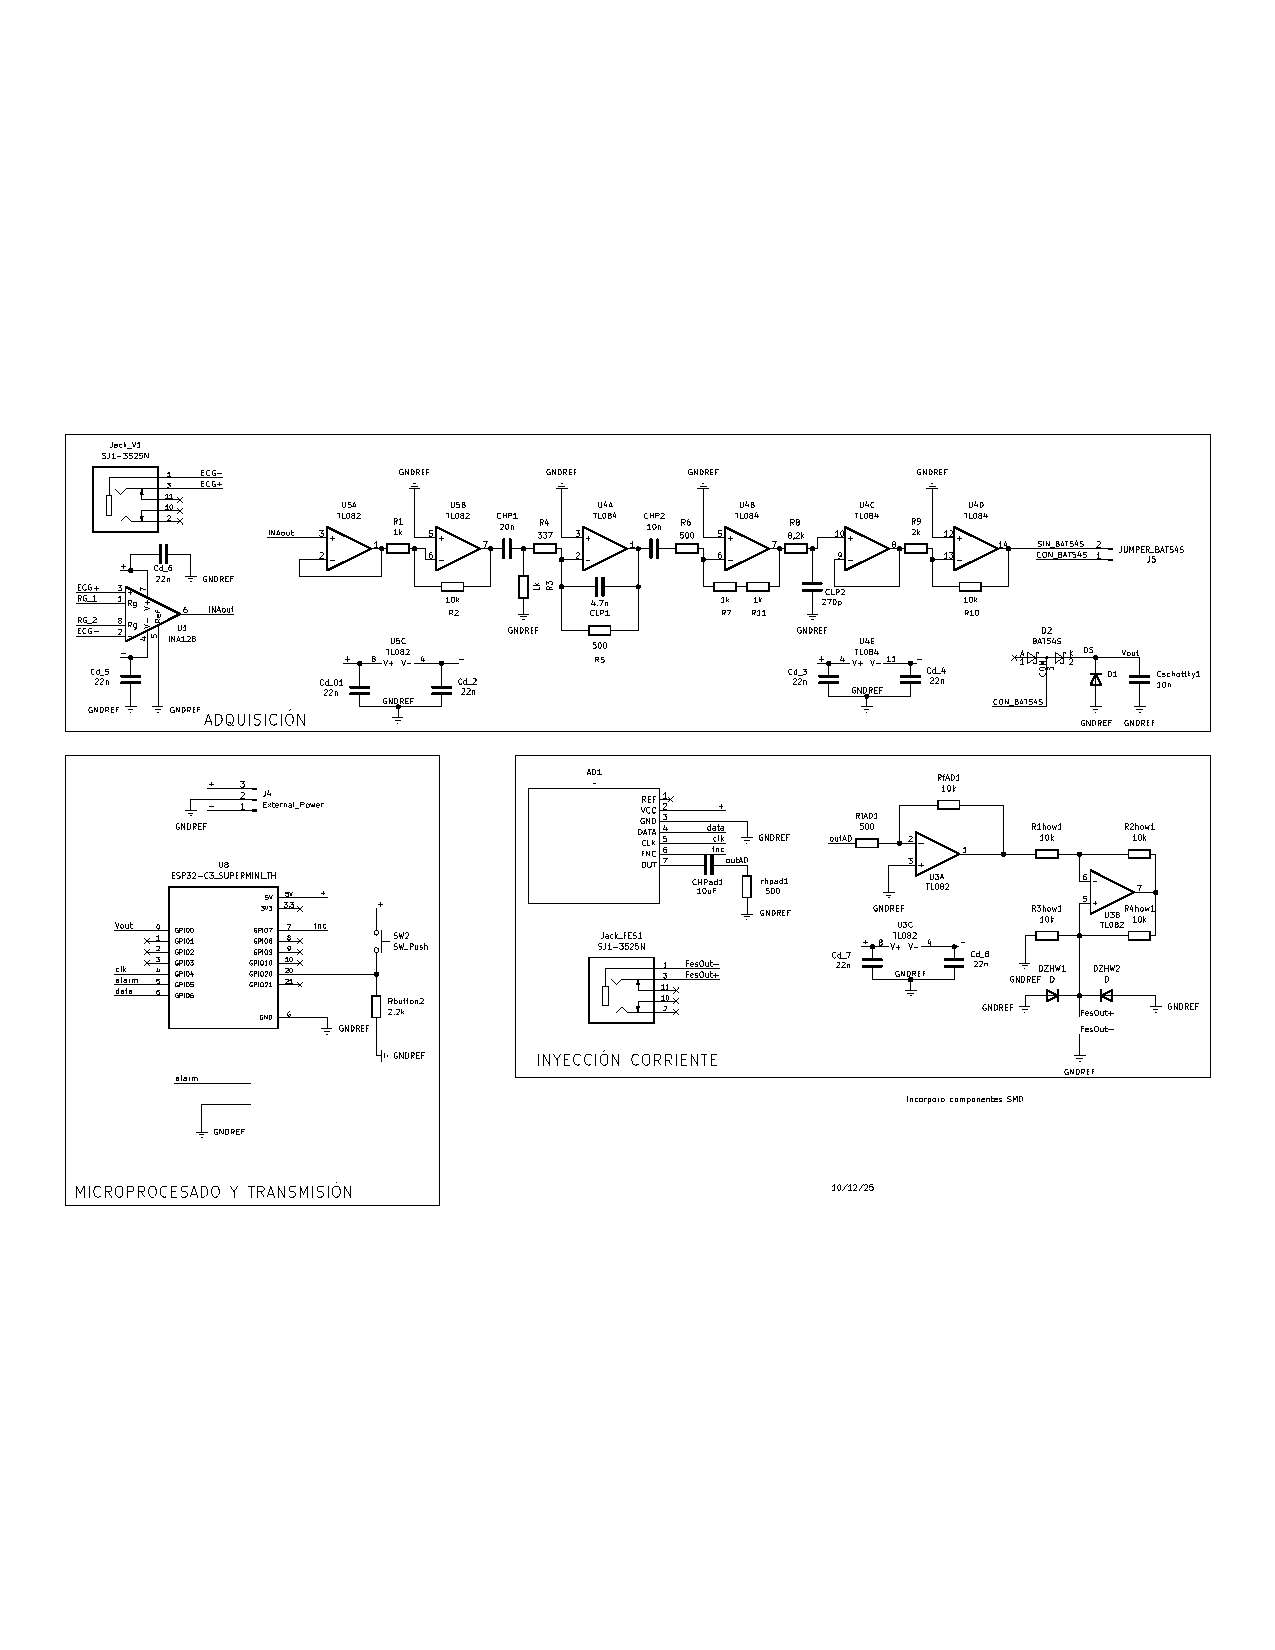
\includegraphics[page=1,viewport=473.68 442.27 577.75 492.11,clip,width=0.48\textwidth]{figuras/esquema_circuito.pdf}
    \caption{Conexiones de selección en J5 y bloque detector con salida Vout.}
    \label{fig:acq_detector}
\end{figure}

La tensión en Vout se aplica al ADC del ESP32-C3. La magnitud digitalizada representa el
nivel entregado por el detector y se utiliza para estimar la amplitud
de la señal anterior a la rectificación. La relación entre ambas tensiones se caracteriza
experimentalmente considerando la caída del diodo, la carga y el ripple. Esa caracterización,
junto con la ganancia de la cadena de adquisición, permite establecer la conversión de la lectura del ADC
a impedancia. 


\clearpage
\subsection{Digitalización, procesamiento y comunicación de datos}

\subsubsection{Muestreo y filtrado digital de la señal}

La tensión continua entregada por el detector de envolvente se digitaliza con el conversor
analógico--digital del ESP32-C3, de 12~bits de resolución y configurado con una atenuación de entrada
de 11~dB para admitir señales de hasta aproximadamente 3,3~V. Para compensar la no linealidad propia de
este conversor, la lectura se realiza mediante la función de calibración de fábrica del fabricante en
lugar de una conversión lineal directa. El microcontrolador muestrea esta entrada a una frecuencia
aproximada de 700~Hz y promedia bloques de 192 muestras consecutivas, obteniendo así un valor de tensión
continua cada 274~ms aproximadamente, a partir del cual se calcula un valor bruto de impedancia mediante

\begin{equation}
    Z=\frac{V_{\mathrm{pp}}}{I_{\mathrm{iny}}\,G},
\end{equation}

donde $V_{\mathrm{pp}}$ es la tensión pico a pico reconstruida a partir de la lectura continua y de la
caída del diodo Schottky, $I_{\mathrm{iny}}$ la corriente nominal inyectada y $G$ la ganancia total de la
etapa receptora.

Dado que el llenado vesical evoluciona en una escala de minutos, se priorizó la relación señal--ruido
por sobre la velocidad de respuesta al diseñar el filtrado digital de $Z$. En primer lugar se aplica un
filtro de mediana móvil de ventana 5, que descarta transitorios aislados sin difundir su efecto sobre las
muestras vecinas; sobre su salida se aplica luego una media móvil de 12 muestras, que reduce el ruido de
naturaleza gaussiana remanente. El orden de esta cascada es relevante, ya que promediar antes de aplicar
la mediana mezclaría cualquier transitorio con las muestras adyacentes y degradaría el filtrado
posterior. Las primeras cinco muestras de cada medición se descartan como período de estabilización, con
el fin de que el transitorio de arranque no contamine el valor basal de referencia $Z_0$, que se fija con
la primera muestra válida obtenida a continuación.

\subsubsection{Comunicación inalámbrica y protocolo de control}

El ESP32-C3 opera como punto de acceso WiFi propio, de modo que el equipo no depende de infraestructura
de red externa y mantiene una dirección IP fija. La comunicación con la interfaz gráfica se establece
mediante \textit{WebSocket} sobre un puerto dedicado, protocolo que permite mantener abierto un canal
bidireccional entre el microcontrolador y el navegador. El firmware transmite periódicamente un mensaje
con tres valores: la impedancia filtrada $Z$, la tensión pico a pico reconstruida a la salida del
receptor y la tensión continua leída directamente en el pin del conversor, esta última incluida para
poder contrastarla experimentalmente con un instrumento de banco. La interfaz, a su vez, envía comandos
de texto que gobiernan el inicio y la detención de las mediciones y permiten consultar el estado del
equipo (intensidad de señal, memoria disponible e impedancia vigente) sin interrumpir la adquisición en
curso. Un mecanismo de \textit{heartbeat} cierra automáticamente las conexiones que dejan de responder,
evitando que sesiones de navegador inactivas degraden la transmisión.

\subsubsection{Máquina de estados y control físico}

El firmware implementa una máquina de estados con los modos \textit{Inactivo} y \textit{Midiendo}; la
evaluación de los umbrales de alarma se realiza en la interfaz y no en el microcontrolador, que actúa
como un sensor de propósito simple. El equipo puede iniciarse y detenerse tanto desde la interfaz como
mediante un botón físico. Para evitar que un roce accidental o una vibración interrumpan una sesión de
medición prolongada, se estableció una asimetría deliberada en el antirrebote: iniciar una medición
requiere sostener el botón durante 80~ms, mientras que detenerla requiere un sostenido de 1,5~s,
confirmado con una señal sonora. Cada inicio de medición reinicializa el generador de señales como medida
defensiva frente a eventuales fallos de arranque de la señal sinusoidal.

\subsection{Interfaz de usuario, alarmas y registro de sesiones}

\subsubsection{Calibración del basal y configuración de alarmas}

El valor basal de impedancia $Z_0$ puede establecerse de dos maneras. De forma automática, la interfaz
toma la mediana de las primeras muestras recibidas al iniciar una medición, reduciendo la influencia de
transitorios iniciales sobre la referencia. De forma guiada, un asistente de calibración de cuatro pasos
permite registrar secuencialmente la impedancia con la vejiga vacía ($Z_0$) y, en una instancia
posterior, con la vejiga llena ($Z_f$), calculando a partir de ambos valores la caída relativa en
decibeles

\begin{equation}
    \mbox{Ca\'{\i}da (dB)} = 20\log_{10}\left(\frac{Z_0}{Z_f}\right),
\end{equation}

magnitud ya empleada para caracterizar el desempeño del prototipo anterior.

A partir del basal fijado, el usuario puede configurar una alarma según tres criterios excluyentes entre
sí:

\begin{itemize}
    \item \textbf{Valor absoluto:} la alarma se dispara cuando la impedancia medida cae por debajo de un
    valor fijo definido por el usuario.
    \item \textbf{Porcentaje del basal:} la alarma se dispara cuando la impedancia cae por debajo de un
    porcentaje del valor $Z_0$.
    \item \textbf{Diferencia respecto del basal:} la alarma se dispara cuando la caída de impedancia
    respecto de $Z_0$ supera una magnitud fija, expresada en ohmios.
\end{itemize}

En los tres casos, la condición de disparo incorpora una banda de histéresis proporcional al umbral
configurado, de modo que fluctuaciones pequeñas alrededor del umbral no generen activaciones y
desactivaciones repetidas de la alarma. Al dispararse, la interfaz emite un aviso visual persistente y
envía una orden al microcontrolador para activar un zumbador, que el paciente puede silenciar mediante el
botón físico del equipo.

\subsubsection{Registro de sesiones y exportación de datos}

Cada sesión de medición puede asociarse a una ficha de paciente y a un conjunto configurable de variables
contextuales (por ejemplo, ingesta de líquidos, registrada acumulando los eventos marcados durante la
medición). Al finalizar una sesión, los datos --curva de impedancia, eventos marcados por el usuario y
variables contextuales-- pueden exportarse en formato PDF, CSV o de texto plano, y opcionalmente
sincronizarse con una base de datos en la nube mediante una cola de reintento que indica en la interfaz
el estado de cada escritura. Este mecanismo constituye la base para la construcción de la base de datos
experimental descripta en los objetivos del trabajo.

\section{Resultados}
\label{sec:resultados}

\subsection{Caracterización experimental de la cadena analógica}
Se registraron con osciloscopio las amplitudes en distintos puntos de la placa. La Tabla~\ref{tab:amplitudes_medidas} registra los valores 
medidos. Las amplitudes anteriores al detector se expresan de pico a pico.

\begin{table}[htbp]
    \centering
    \caption{Amplitudes medidas con osciloscopio en la placa 1.}
    \label{tab:amplitudes_medidas}
    \begin{tabular}{lr}
        \hline
        Punto de medición & Tensión pico a pico (mV) \\
        \hline
        Salida del seguidor U5A & 14 \\
        Salida del amplificador inversor U5B & 158 \\
        Salida del primer filtro inversor U4A & 160 \\
        Salida del pasaaltos activo U4B & 510 \\
        Salida del pasabajos y seguidor U4C & 330 \\
        Salida del amplificador final U4D & 1450 \\
        \hline
    \end{tabular}
\end{table}

A la salida del detector se registraron 556~mV. Para la señal de 1,45~V pico a pico
anterior al detector, suponiendo una senoide centrada en cero, el valor de pico es
725~mV. La diferencia entre ese valor y la tensión detectada es 169~mV.

En la etapa inversora previa a la fuente de Howland se midieron 3,22~V pico a pico,
con una resistencia de entrada de 1~k$\Omega$, como se indicó en metodología.





\section{Conclusiones}



\printbibliography


\clearpage
\appendix
\section{Esquema electrónico del circuito}
\label{anexo:esquema_circuito}

La Figura~\ref{fig:esquema_circuito_completo} reproduce el esquema suministrado, con los
bloques de adquisición, inyección de corriente y microprocesado y transmisión.
En el bloque de adquisición se muestran también las conexiones de alimentación de los TL082
y TL084 y los capacitores de desacoplamiento de 22~nF entre los rieles y la referencia de masa.

\begin{figure}[htbp]
    \centering
    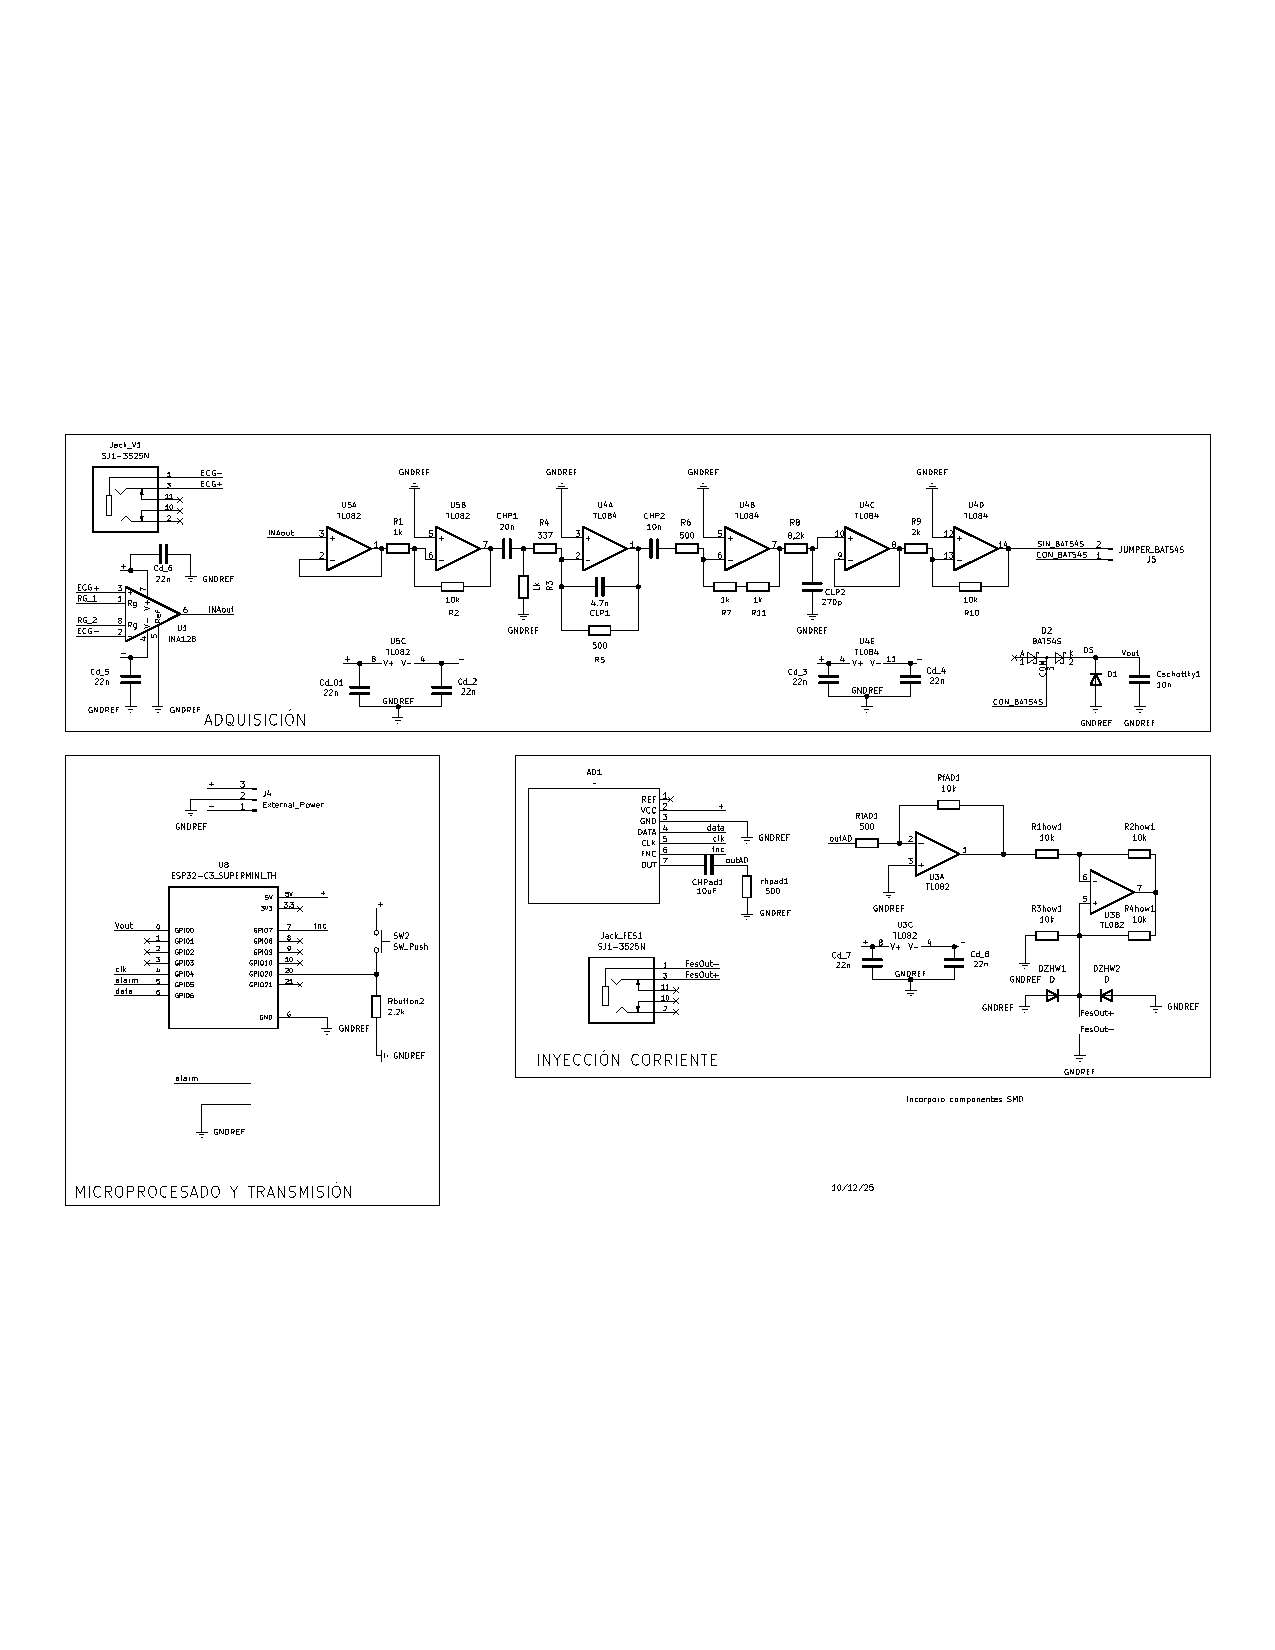
\includegraphics[page=1,viewport=30.69 211.35 581.76 583.77,clip,width=1.0\textwidth]{figuras/esquema_circuito.pdf}
    \caption{Esquema electrónico general. Los detalles del acondicionamiento se presentan ampliados en la sección de adquisición.}
    \label{fig:esquema_circuito_completo}
\end{figure}

\end{document}
